\documentclass{swathesis}
\usepackage{amsmath}
% \PassOptionsToPackage{final}{graphics}
% \documentclass[draft]{swathesis}
\KOMAoptions{
  DIV=9,
  BCOR=6mm
}
% \input{system}
\newboolean{thesis}
\setboolean{thesis}{true}
% \setboolean{printmode}{true}
% \input{style}
\hyphenation{Small-talk in-ter-me-di-ate Kohl-beck-er how-ev-er o-ri-ent-ed hand-ling}

\iffalse
\newcommand{\eg}{e.\hairspace{}g.\xspace}
\newcommand{\Eg}{E.\hairspace{}g.\xspace}
\newcommand{\Ie}{I.\hairspace{}e.\xspace}
\newcommand{\ie}{i.\hairspace{}e.\xspace}
\else
\newcommand{\eg}{e.\hairspace{}g.,\xspace}
\newcommand{\Eg}{E.\hairspace{}g.,\xspace}
\newcommand{\Ie}{I.\hairspace{}e.,\xspace}
\newcommand{\ie}{i.\hairspace{}e.,\xspace}
\fi
\newcommand{\cf}[1]{cf.\,{#1}\xspace}

\newacronym{api}{application programming interface}
\newacronym{clr}{Common Language Runtime}
\newacronym{com}{Component Object Model}
\newacronym{cop}{context-oriented programming}
\newacronym{http}{the Hypertext Transfer Protocol}
\newacronym{iaas}{Infrastructure-as-a-Service}
\newacronym{ipc}{Inter-process communication}
\newacronym{jdi}{Java Debugger Interface}
\newacronym{jvmti}{Java Virtual Machine Tools Interface}
\newacronym{jit}{just-in-time}
\newacronym{json}{JavaScript Object Notation}
\newacronym{jvm}{Java virtual machine}
\newacronym{lcs}{longest common sub-sequence}
\newacronym{osi}{Open Systems Interconnection}
\newacronym{paas}{Platform-as-a-Service}
\newacronym{rest}{REpresentational State Transfer}
\newacronym{soa}{Service-oriented Architectures}
\newacronym{tcp}{Transmission Control Protocol}
\newacronym{udp}{User Datagram Protocol}
\newacronym{uml}{Unified Modeling Language}
\newacronym{uuid}{universally unique identifier}
\newacronym{vcs}{version control system}
\newacronym{vm}{virtual machine}
\newacronym{xhr}{XMLHttpRequest}

%%% this is for discriminating thesis vs, eg, tr
\ifthenelse{\boolean{thesis}}{
% \newcommand{\we}{I\xspace}
% \newcommand{\We}{I\xspace}
\newcommand{\we}{we\xspace}
\newcommand{\We}{We\xspace}
\newcommand{\work}{thesis\xspace}
}{
\newcommand{\we}{we\xspace}
\newcommand{\We}{We\xspace}
\newcommand{\work}{work\xspace}
}

\newcommand{\CPP}{C\kern-.05em\raise.15ex\hbox{+\kern-.05em+}\xspace}
\newcommand{\CS}{C\kern-.02em\raise.1ex\hbox{$\#$}\xspace}
\newcommand{\Cone}{C{\liningnums{1}}\xspace}
\newcommand{\HotSpot}{HotSpot\texttrademark{}\xspace}

%%% Local Variables: 
%%% mode: latex
%%% TeX-master: "thesis"
%%% End: 

\addbibresource{library.bib}

\newboolean{closures}
\setboolean{closures}{false}


%\usepackage{showframe}
 \errorcontextlines=99

\ifthenelse{\boolean{thesis}}{
\usepackage{titlepage}
\TitlePageStyle[
subject=master,degree={Master of Science},
]{hpi-swa}

\supervisors{%
Prof.\,Dr.\,Robert Hirschfeld \and %
Michael Perscheid%
}
}{}

% \setdate{2012}{04}{05}
% \date{\datedate}
\extratitle{\raggedleft Felgentreff, \\Debugging Distributed Applications\par}
\title{Comparison, Replay, and Refinement of Communication Traces for
  Debugging Distributed Failures}
% \subtitle{}
\author{Tim Felgentreff}

\begin{document}
\frontmatter
\maketitle
\begin{abstract}
  An increasing number of companies build their business on
  distributed Web applications. Hosting providers respond to that
  demand and made it easier to deploy systems that spread across
  multiple services. However, this trend has outpaced the development
  of adequate debugging tools and developers still have to rely on an
  improvised patchwork of symbolic debuggers and printf debugging to
  find failure causes.

  Consequently, observing and debugging failures in distributed
  applications is laborious and time consuming. As multiple processes
  execute in parallel, developers cannot systematically stop and
  inspect the entire system. Although processes are implemented in
  different languages, and often tightly coupled, debugging tools that
  span across processes and languages are practically
  non-existent. Instead, developers have to use different debugging
  techniques to inspect each process sequentially. This makes it hard
  to reason about causality, because the network communication changes
  when debugging a process. That may lead to failures that occur in
  deployed systems, but that developers cannot reproduce locally.

  This work presents an integrated method to support debugging of
  distributed systems in four steps: First, we continually trace
  network communication to have accurate data about event order if a
  failure occurs in a deployed system. Second, we compare
  communication patterns heuristically to identify anomalous
  differences and guide developers in search of failure causes. Third,
  we replay failing network schedules to reproduce failures in a local
  test environment. Finally, we refine the traced data during replays
  and connect network events to code locations. We present network
  events and code within one tool, so developers can use both levels
  of abstraction for debugging.

  We show how our approach can be used to inspect failures in
  distributed systems that would be hard to debug with traditional
  approaches.
\end{abstract}

\begin{zusammenfassung}
  Die Zahl der Firmen, die als Teil ihres Geschäftes verteilte Web
  Anwendungen entwickeln, nimmt zu. Anbieter zur Bereitstellung von
  Servern bedienen die steigende Nachfrage, und erleichtern den
  Einsatz von Systemen die sich über mehrere Dienste hinweg
  erstrecken. Dieser Trend jedoch schreitet schneller voran, als die
  Diagnoseprogramme für diesen Einsatzbereich weiterentwickelt werden,
  weshalb Entwickler noch immer mit symbolischen Fehlersuchwerkzeugen
  und Protokollierung arbeiten müssen, um Fehler zu finden.

  Folglich ist das Beobachten und Beheben von Fehlern in verteilten
  Systemen noch immer mühselig und zeitaufwendig. Da mehrere Prozesse
  parallel laufen, können Entwickler nicht das gesamte System zur
  Untersuchung anhalten. Obwohl Prozesse in mehreren Sprachen
  implementiert, und eng gekoppelt sind, gibt es praktisch keine
  Werkzeuge, die über Prozess- und Sprachgrenzen hinweg
  funktionieren. Stattdessen müssen Entwickler verschiedene
  Fehlersuchtechniken für jeden Prozess einzeln anwenden. Das
  erschwert es ihnen, kausale Zusammenhänge zu verstehen, da sich das
  Kommunikationsverhalten ändert, wenn einzelne Prozesse untersucht
  werden. Das kann dazu führen, dass Fehler, die im Produktivsystem
  auftreten, von Entwicklern lokal nicht reproduziert werden können.

  In dieser Arbeit wird eine Methode zur Fehlersuche in verteilten
  Systemen präsentiert, welche die folgenden vier Schritte umfasst:
  Zunächst wird fortwährend die Kommunikation im Netzwerk
  aufgezeichnet, um im Falle eines Fehlers im Produktivsystem den
  Entwicklern akkurate Ereignisdaten bereitzustellen. Daraufhin werden
  diese Daten mithilfe einer Heuristik auf Anomalien in den
  Kommunikationsmustern hin untersucht. Weiterhin werden diese Daten
  zur Wiedergabe der Kommunikation in einem Entwicklungssystem
  genutzt. Schließlich werden die aufgezeichneten Daten während der
  Wiedergaben verfeinert, und so die Netzwerkdaten mit dem Quelltext
  assoziiert. Beides wird in einem Werkzeug präsentiert, sodass
  Entwickler beide Abstraktionsebenen zur Fehlersuche nutzen können.

  Wir zeigen wie unsere Methode genutzt werden kann, um Fehler in
  verteilten Systemen zu finden, die mit traditionellen Ansätzen nur
  schwierig untersucht werden können.
\end{zusammenfassung}
 

%%% Local Variables: 
%%% mode: latex
%%% TeX-master: "thesis"
%%% End: 

%% !TEX root = Stolpe_2018_Thesis.tex
% !TEX encoding = UTF-8
\begingroup
\let\raggedsection\centering

\chapter*{Acknowledgments}
\label{cha:acknowledgments}
\endgroup
\begin{quotation}
  \noindent I owe everything to my cat.
\end{quotation}
%%% Local Variables:
%%% mode: latex
%%% TeX-master: "Stolpe_2018_Thesis"
%%% coding: utf-8
%%% End:

\tableofcontents
\listoffigures
% \listoftables
% \lstlistoflistings
\listofacronyms %
\mainmatter

\chapter{Introduction}
\label{cha:introduction}

From its beginnings in the 1990s, the Web has become an important
application platform in less than one and a half decades. Industry
surveys indicate that an increasing number of companies develop
distributed Web applications as a core part of their
business~\cite{kondo2009cost,EYPaaSSurvey2012}. However, many of those
applications are not written with distributed systems middleware to
handle communication between services. Instead, developers improvise
their own communication interfaces. This is error-prone and
complicates integration~\cite{Nadiminti}.

Distributed applications are especially prone to software
failures. Recent studies~\cite{Ballou2008,Tassey2002} show a relative
increase in code problems, hidden dependencies, and accidental
complexity when integrating multiple systems. Different systems may
provide different network interfaces and developers need to understand
their utilization and implicit assumptions. Different systems also run
different frameworks and programming languages, so that developers
need help to associate observed network communication with code
locations. This additional complexity makes it harder for developers
to reason about the system as a whole, thus, they are more likely to
introduce defects~\cite{zeller2009programs}. Debugging the resulting
failures is hard, and we have identified four primary problems that
developers face with current approaches and tools.

First, reliably reproducing failures is hard. Since distributed
systems execute in parallel, a global event order is difficult to
establish and may vary non-deterministically across
executions~\cite{lamport1978time}. Such variance depends on the
physical connections between the servers. The development setup will
differ from deployment and, thus, network delays and probabilities for
non-deterministic behavior also differ. Consequently, developers may
not be able to trigger some failures during development that occur in
deployment, or such failures may occur so rarely that it is impossible
to debug them effectively, because developers cannot reliably
reproduce them.

Second, developers cannot easily distinguish between causes and
effects. Many developers rely on systematic logging to understand
failures that only occur during
deployment~\cite{zeller2009programs}. However, isolated event logs are
poorly suited to create a global view on the events in a distributed
application. The ability to reason about global event order is
necessary for humans to understand causality in a
system~\cite{lamport1978time}. Understanding the cause of a failure is
essential for fixing it correctly.

% Consider a search engine. For a small scale engine, developers can
% control data storage, transactions, and database connections. On the
% Internet, the primary communication protocol is \ac{http} which limits
% in the amount of control developers have over their systems'
% connections. Non-atomic data updates usually cannot be wrapped in
% transactions. Storage services on the Web cannot provide transactions
% to thousands of users in parallel. Parallel \ac{http} request are each
% stateless and provide no guaranteed ordering. Thus, developers can
% rely less on the underlying infrastructure and require debugging tools
% work in a distributed setting.

Third, developers cannot easily inspect execution on servers in the
system. With symbolic debuggers, programmers inspect execution state
and behavior to find anomalies that may have caused a
failure. Symbolic debuggers enable them to stop execution and
interactively inspect the program's state. However, in a distributed
system, developers need to inspect state across multiple servers,
which execute in parallel. Symbolic debuggers are tailored towards
systems under developer control, but not all parts of a distributed
system provide that kind of control. Stopping servers with a debugger
to inspect the execution state is not feasible during deployment and
external services may not provide any debugging mechanism.

Finally, different frameworks and programming languages on several
servers force developers to apply multiple debugging
tools. Consequently, developers cannot debug and inspect the
distributed system as one. Instead, they have to treat each system
separately, because current debugging tools cannot connect and
synchronize with others. Support for debuggers that work across
multiple servers and languages is virtually non existent.

Due to these problems, debugging failures in distributed systems,
especially non-deterministic failures, is a time-consuming task. It
usually consists of aggregating various forms of log files, debug
output, and \ac{api} documentation for the employed services, and then
debugging on an equivalent, local system to infer possible
problems. Symbolic debuggers cannot be used in distributed
applications, because they only support independent analysis of
individual processes and require full control over those.

Tool support for network observation, log aggregation and debugging
across different systems is virtually non-existent. Yet, to improve
programmer productivity, providing adequate debugging tools is a key
ingredient, as without them, debugging is a manual, time-consuming
task~\cite{Dinning1990}.

We argue that there is a need for debugging tools that target
distributed, heterogeneous systems which are not entirely under
developer control. Architectural patterns for the these kinds of
systems, such as \ac{soa} and \ac{rest}; and hosting services, such as
\ac{paas} and \ac{iaas}, are relatively new phenomena---the first
comprehensive description of \ac{soa} was in 2005~\cite{Erl2005}. For
that reason, much of the work in this area is still not aimed at the
specific challenges of debugging distributed applications. Developers
of these systems need tools that provide a means to record and replay
events consistently across multiple servers. The tools should
furthermore guide developers towards anomalous differences across
multiple executions, so developers can reason about causality in the
system. Finally, such a tool should allow developers to cope with
multiple frameworks and languages, as they are common in distributed
applications.

\section{Approach}
\label{sec:approach}

In this work we present an approach for integrated debugging in
distributed applications, targeted specifically at Web development,
but extensible to other kinds of applications with similar
problems. Our approach---Replay-driven Fault Navigation---combines
state of the art techniques in the area of record and replay to
eliminate of non-determinism, distributed program comprehension, and
statistical debugging.

To allow debugging of non-deterministic failures, we present a tracing
approach for unified monitoring of systems. We continuously monitor
the live system and record enough data to allow reproducing relevant
program state at a later time. Our monitoring imposes little overhead
so it does not disturb execution unduly and can stay enabled during
deployment. We analyze the recorded data and correlate it to failures
to determine causes and effects. Network schedules are treated as
sequences of send and receive events between pairs of servers. Our
heuristics assign cause probabilities to sub-sequences of the recorded
network schedules, to guide developers during debugging. Developers
can replay such event sequences with our network scheduler and
iteratively refine recorded execution data for inspection. The
scheduler is an intermediate layer that controls how network events
pass between the application code and the framework. It blocks or
stalls events to change the order in which they pass in and out of the
application to match the recorded sequence. We correlate the network
data with source code and present both in a unified debugging tool, so
developers can debug at either level of abstraction and correlate
source code across servers and languages.

The advantages of our approach over traditional stop-the-world
symbolic debuggers are: the impact on the runtime behavior is kept at
a minimum, the technique can be applied to the live system,
eliminating the need for a test setup, and the debugging tools can
help developers to logically connect source code locations across
different servers.

To our knowledge, the presented approach is unique in that it
explicitly tries to support debugging across different languages and
system with one integrated approach. Work on understanding and
debugging distributed systems has been on-going for some
time~\cite{Parker1983} and the state of the art has solutions for each
part of Replay-driven Fault Navigation, but no integrated solution
exists that we are aware of.

\section{Outline}
\label{sec:outline}

This work is structured as follows: in \autoref{sec:requ-based-distr},
we discuss the problem domain on a small example. We highlight
challenges faced by developers when working with current debugging
techniques. In \autoref{cha:solution-design}, we present our four-step
approach to those challenges, and how that approach could work in
different languages and deployment scenarios. In
\autoref{cha:implementation}, we discuss an implementation of
Replay-driven Fault Navigation in Smalltalk. Finally in
\autoref{cha:evaluation}, we use the initial example and a larger
application adapted from an industrial system to evaluate our tool in
comparison with contemporary techniques. In
\autoref{cha:related-work}, we discuss related work and present our
conclusions in \autoref{cha:conclusion}.

%%% Local Variables: 
%%% mode: latex
%%% TeX-master: "thesis"
%%% End: 

\chapter{Request-based Distributed Applications}
\label{sec:requ-based-distr}

A distributed application consists of a number of processes running on
one or more servers that are communicating over a network, for the
purposes of this work, the Internet. Such applications are especially
prone to software bugs~\cite{Ballou2008}. Software bugs are defects in
a program that developers introduce through an error in thinking. If
the defective code is executed it causes an infection of the execution
state. If this infection propagates to other states, it may eventually
become visible in form of a failure~\cite{zeller2009programs}. In this
work we focus on debugging distributed Web applications, but our
approach is applicable to other distributed applications as well.

Web applications are applications accessible through a Web browser,
with, at least, a client-side component for interaction and a
server-side component for data storage. Clients are written in
JavaScript to run in the browser, and the server components may use
any programming language. Many Web applications use \ac{http} as
transfer protocol, with event-loops to handle asynchronous
communication. The reason for this is the single-threaded nature of
JavaScript in modern browsers. In the absence of multiple threads or
processes, event loops are the only option to process multiple network
events in parallel on the client. However, developers increasingly
employ event loops for server implementations as well. Event loops
avoid spawning large numbers of threads or processes that are---due to
the potentially high network latencies across wide-area
network---waiting for IO most of the time. Web applications have at
least a client and a server component, but both often communicate with
other services. These, \emph{asynchronous request-based, distributed,
multi-language applications}, are the subset of applications this work
is aimed at.

The communication patterns of many distributed systems on the Web can
be described using \ac{uml} sequence
diagrams~\cite{rumbaugh2004unified}. In a sequence diagram, each
server is an entity with a lifeline for request handling, and receives
and sends asynchronous requests. Even though \ac{http} is a
synchronous protocol, if we regard both requests and responses as
asynchronous requests, we can treat servers that handle parallel
request using any mechanism as a single thread with only asynchronous
request-handling using event-loops.

\section{Motivating Example}
\label{sec:motivating-example}

We now present an example system that uses asynchronous communication
between multiple servers. Meta-crawlers are a type of Web search
engine that connect to other search engines. Meta-crawlers combine
information from other sources and provide a unified interface to
interact with that information. For example, flight booking systems
that offer multiple airlines connect to the systems of the different
airlines and provide a unified search and booking interface to
customers. Meta-crawlers such as these offer more than just search
across multiple providers, they provide additional services for
comparing prices, comparing seating options, or booking flights.

\subsection{System Description}
\label{sec:system-description}

We have built a system that implements such a meta-crawler and is
connected to a service providing fake airline data. It consists of a
Web site that allows the user to search for and reserve flights from
an origin to a destination on a specific date. The server serving the
Web site communicates with a cache. That cache provides flight
information and caches it for a certain amount of time. Such flight
information includes flight numbers, origin and destination of
flights, information about intermediate airports for a flight, as well
as pricing and available seats. This cache, in turn, connects to a
flight-data generator service that stands in for the airlines
providing information about their scheduled flights. All communication
is done via \ac{json}\footnote{JavaScript Object Notation\\
\url{http://www.ietf.org/rfc/rfc4627.txt}\\ accessed July 25,
2012}. The setup for this system is shown if
\autoref{fig:flyhehe-setup}, with the arrows indicating data
direction.

An intermediate query and cache service is an optimization that
meta-crawlers use, which avoids having to query the data sources
directly on each user request. Querying on each request is undesirable
due to network latencies and because data providers usually limit the
number of queries per time unit that meta-services can send to save
bandwidth and processing time. However, caches introduce the problems
of stale data and cache invalidation. Prices for seats on airplanes
usually rise as the flight date approaches, and as increasingly fewer
seats are available. Consequently, in order to create a reservation,
flight booking systems either cannot guarantee the exact prices for
their results, or they have to invalidate their caches and query for
current data at the time of reservation.

\begin{figure}
  \centering
  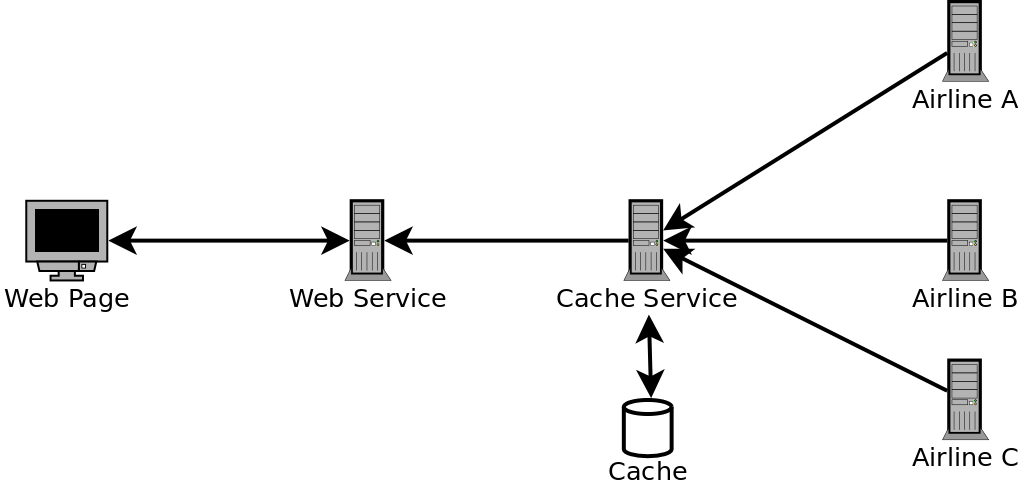
\includegraphics[width=0.7\linewidth]{flyhehe-setup}
  \caption{Flight Meta-Crawler Demo Setup}
  \label{fig:flyhehe-setup}
\end{figure}

\subsection{Failure Scenarios}
\label{sec:failure-scenarios}

Consider two customers on the meta-crawler Web page at the same
time. Both are looking for flights from Berlin to Amsterdam, as shown
in \autoref{fig:flyhehe}. The results of their search will be served
from the cache, and may not be the most recent data from the
respective airlines. If both customers try to reserve seats on flight
\emph{LH1009} at roughly the same time, different things may happen.

First, depending on the geographical location of both users with
respect to our system, the request for reservation may take some time
to reach the server. Depending on the time difference, one reservation
may complete entirely before the other request even arrives at the
server. As we have said above, in order to create a guaranteed
reservation, the Web server has to query the airline data---or, in our
case, the fake airline data generator---for the most recent rates and
available seats. Let us assume that the cache data was current and the
first reservation request can be fulfilled at the displayed rate of
156 EUR. By the time the second request for reservation arrives at the
Web server, the number of available seats has thus gone down to one,
which means the prices has gone up as the airline adjusts pricing
depending on available seats. Thus the second reservation can also
complete, but only at a higher rate.

Second, it may be that both requests for reservation \emph{arrive} at
our server at the same time, and are served in parallel. This leads to
a race condition for which we cannot deterministically decide which
one of the users receives the lower rate and which one the higher
rate. Either way, we, as the provider of the meta-service, do not want
to end up reserving two seats and receiving only the lower rate from
both customers, because in that case, depending on our and the
airlines' terms of service, we may have to pay the price difference or
a fine, which may not be a sustainable way to make business. At the
same time, as a customer, we do not want to create a binding
reservation at any other rate than the one shown on the Web site at
the time of our click on the \emph{Reserve Seat} link.

\begin{figure}
  \centering
  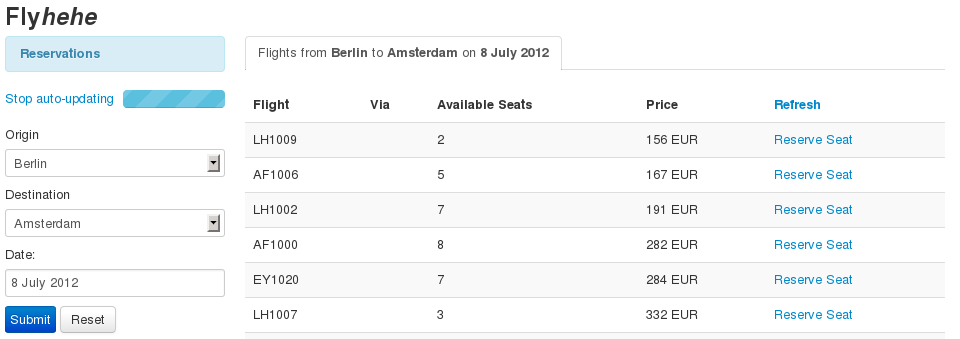
\includegraphics[width=\linewidth]{flyhehe}
  \caption{Flight Meta-Crawler Demo System}
  \label{fig:flyhehe}
\end{figure}

There are a number of challenges for the developers of such a
system. First, they have to understand the communication patterns that
may arise in production, with parallel access to the Web site, cache,
and airline data. They have to implement ways to deal with data races
and non-determinism caused by network delays. To do that, they have to
understand how non-determinism may lead to undesired states in their
application, such as making a wrong reservation. To verify their
solutions, they need a way to reliably reproduce problems and test
them. Finally, they need to understand how communication between two
systems tightly couples them at the implementation level, which means
they have to understand how changes to the code in one system may
impact that systems' ability to communicate with the others.

\subsection{From Bug Report to Failure}
\label{sec:from-bug-report}

A bug is an expression of a defect as a visible failure in the output
of a system. To fix a bug, developers have to understand the failure,
find the underlying defect, and remove it. Imagine the following bug
report for our flight booking system:

\begin{quote}
  Sometimes, when I try to book a flight on your website,
  it is added to my cart just fine, but with a different price than what
  it was in the list when I clicked it.
\end{quote}

This particular bug report is at a high abstraction level, as it
describes only user-facing input and effects. For such bug reports,
the first step towards fixing them is to reproduce them. Second,
developers should write a minimal piece of executable code that
reproduces the failure, so they can easily check their attempts at a
fix. Then the actual process of debugging can begin, which will
eventually make the test case pass.

These steps can be time-consuming, especially for very abstract bug
reports. Tools such as \emph{ReCrash}~\cite{Artzi} attempt to generate
test cases automatically, but can only do so for deterministic
failures. The above bug report contains the word "sometimes",
indicating a degree of non-determinism. That non-determinism may have
a number of causes. In this case, it may be that the user attempts to
book flights slightly differently without noticing. There may be
conditions in the environment, from browser bugs to transient hardware
failures, that cause the issue to only appear sporadically. Or there
may be non-determinism in the Web server implementation or the network
communication.

To approach non-determinism during debugging, developers have to check
each possible cause and try to eliminate it. Most of these causes,
including network communication, are difficult to reproduce faithfully
outside the live system. Unit tests are likely to be too low-level to
expose complex interactions, and acceptance tests running in a test
setup experience different conditions if the test setup is not
similar enough to the live system. Developers cannot with certainty
know whether a test setup sufficiently models the live system to
reproduce a given failure.

Given the above bug report and its possible causes, developers at some
point have to inspect the network communication schedule if no other
cause can be found.

\paragraph{Scripted Diagnoses}
\label{sec:scripted-clients}

Instead of acceptance or unit tests in controlled test environments,
developers may employ \emph{system diagnoses} as "test cases" to
simulate user input against the live system. Oftentimes those are
simple scripts simulating a browser's communication with the Web
page. This enables developers to include the circumstances under which
the bug occurred in the test. Even if the bug only occurs "sometimes",
repeated execution of the system diagnosis will eventually reproduce
it if it is related to varying network schedules.

This is the approach taken by tools such as
\emph{iDNA}~\cite{Bhansali2006} and statistical debugging
approaches. The deployed application is observed over long periods of
time, possibly through multiple occurrences of the failure. If the
failure occurs, as established by the bug report, "sometimes", then
the diagnosis is good enough for Replay-driven Fault Navigation.

\section{Challenges when Debugging in Distributed Environments}
\label{sec:debugg-distr-envir}

In distributed systems such as our flight booking system, developers
face a set of challenges in addition to the challenges of
non-distributed systems. The implementation of each service has to
account for the unreliable network, developers need to understand the
services they communicate with, and how data is represented and shared
between those
services.\\

\begin{description}
\item[Non-determinism] Non-determinism may have different causes: from
  randomness in the implementation, varying shared resource access
  order, to interactions with other processes and the operating system
  schedule and transient faults in hardware. Non-determinism here
  means that for equal inputs, the output and execution speed of a
  program is indeterminate.

  For a distributed system, non-determinism may mean that for an equal
  number and order of messages sent from one server, another server
  may produce different responses. A cause unique to distributed
  systems for this is network latency and request re-ordering. Sending
  a number of \ac{http} requests in one particular order does not
  guarantee its delivery in the same order. This is an instance of a
  leaky abstraction. \ac{http} messages may be broken up into multiple
  \ac{tcp} packets. \ac{tcp} packets may arrive out of order, and are
  collected by the operating system and delivered to applications in
  the original order for a connection. If the \ac{tcp} packets for one
  \ac{http} connection are available, the operating system passes
  those packets to the application, which handles them as \ac{http}
  request. The application does not know that another \ac{http}
  request is on its way that was sent earlier from the point of view
  of the sender. So, if the processing of any request is influenced by
  any other, network latency may introduce non-determinism.

  Network latency varies across network segments. Usually, during
  development, distributed systems are deployed in a test environment
  in an attempt to simulate the distribution properties of the
  deployed system. However, actual network latency during deployment
  is hard to predict, and data races across the network will only
  randomly be reproduced in a test environment. Furthermore, during
  development, \emph{click-races}---the situation when two or more
  users try access a resource simultaneously---can oftentimes not be
  adequately tested. Finally, deployed distributed systems, due to
  ongoing communication, very rarely enter a globally consistent
  state, so proving a system correct for its projected uptime is
  difficult~\cite{Geels2006Replay}. The only predictable way to enter
  consistent states is to shut down and restart the whole system
  regularly, which is not desirable for many systems.
\item[Heisenbugs] Failures that occur only during or change during
  debugging are called \emph{Heisenbugs}~\cite{Gray1986}. They happen
  because the debugging tool, through its observation process, changes
  the runtime behavior of the observed program. For non-deterministic
  failures, this means that introducing logging into the system may
  cause different failures to happen, or the original failure could
  happen much more or much less frequently, or not at all. This makes
  debugging non-deterministic failures harder, because the developer
  cannot be sure that the observed failure is the same as the original
  one.

  Distributed systems exhibit Heisenbugs more often, because network
  access order varies even from slight disturbances, such as the
  operating system scheduler or other processes in the system. Most
  debuggers incur significant overhead~\cite{Corliss2005}, which
  causes equally great disturbances to network access order, which in
  turn may cause Heisenbugs~\cite{Gait1985}.
\item[Languages] When systems run on different machines, or even only
  in different processes, and they communicate not via the language
  calling mechanisms, but rather through foreign-function interfaces,
  shared memory, or network communication, connecting call trees in
  one language to another is a non-trivial task.

  A developer has to find exit and entry points for \ac{ipc} in all
  communicating systems, and relate the input and output data, to
  connect events within one system to another. This task is made more
  difficult by abstractions from the input and output, for example,
  while the operating system will deliver \ac{tcp} packets in order to
  a language runtime, a Web framework will assemble \ac{http} messages
  before passing the data on to the application. If systems use
  different abstractions, one working on the transport layer and the
  other on the application layer, it is hard to determine the
  corresponding communication entry points.
\item[Data Representation] Different languages represent data
  differently. Consequently, different kinds of persistent data
  representation come natural to the language users. Different data
  representations have to be converted into each other, which
  introduces additional complexity and another source for
  bugs. Because the connection between the different systems and the
  data conversion is usually hidden behind libraries and frameworks,
  failures that are caused by incorrect data exchange are hard to
  debug, because developers have to understand multiple systems and
  how they transform the data.

  For example, a web-page will naturally display information to a user
  in a visual manner, using nested \textsc{HTML}-\textsc{DOM} elements
  to express the information content in a user-friendly way. The
  JavaScript code running in the browser will usually, at least
  intermittently, store information as JavaScript objects or in
  \ac{json}. \ac{json} may also be the format used in \ac{http}
  requests to transfer data between the client and the server. On the
  server, the data may again be transformed any number of times
  between different runtimes, backend servers, and databases.
\end{description}
~\\
These properties make debugging distributed systems a laborious
task. We have identified the following four debugging activities to be
especially problematic and in need of a solution.

\subsection{Observation and Logging}
\label{sec:observation-logging}

The need for observation and logging of program state changes has
clearly been recognized in both research and
industry~\cite{Saito2005,altekar2009odr,Stanley2009}. Most Web
frameworks include logging facilities, different log-levels, and
separate logs for access, input, output, erroneous and successful
events. There are full libraries\footnote{Airbrake: The error app 
  \url{https://airbrake.io/pages/home}\\
  accessed June 25, 2012} and frameworks\footnote{Apache log4j
  Logging Services
  \url{http://logging.apache.org/log4j/1.2/index.html}\\
  accessed June 25, 2012}
that provide comprehensive logging facilities to applications.

Distributed system are setup differently during development than at
deployment time. Simulation of distributed systems or parts thereof in
small-scale development deployments, as used at development time of
such systems, allows developers to evaluate system behavior in a
simple setting, relative to the deployment setup. In such development
setups, developers have full control over each server, and the power
to stop and inspect each process at practically any point in the
execution of the distributed system. Apart from such small-scale
setups, developers use full-scale test deployments to provide a more
realistic setting for stress testing critical aspects of the
system. Using setups of varying degree between fully local deployments
and full-scale test environments, developers can control the amount of
realism their code is exposed to.

However, once deployed, distributed systems will over time encounter
situations that could not have been anticipated by the developers,
state changes accumulate, the underlying network topology changes,
and, for successful services, system load and parallelism increases
beyond what could reasonably be
tested~\cite{Geels2006Replay}. Long-running applications may
experience non-deterministic, low-probability failures that develop
over time. Thus, logging data from the deployed system is
indispensable for testing and debugging failures that occur during
deployment.

If problems occur, most logging frameworks have settings on how to
react, by sending emails, checkpointing the running application,
stopping and saving a stack-dump of the program state,
etc. \emph{heartbeat} services regularly check accessibility of
services, existence of error artifacts, or output of logging
frameworks, to filter and notify developers when a problem occurs in
the deployed system.

Logging frameworks and error artifacts are useful for debugging, as
long as only a limited number of frameworks is used. As long as logs
are similar in format and level of abstraction, they can be related to
one another. However, although most frameworks that are used in the
context of networked applications offer logging capabilities, there is
no widely accepted standard for logging information and formats across
languages or frameworks.

\subsection{Understanding and Classifying Observations}
\label{sec:distr-reas}

Given appropriate logging, developers have to review and understand
the logs to determine how to approach a particular bug. This entails
associating parts of a log or particular log entries with
failures. Even for stack traces of single process applications, this
is no easy task, and developers can easily get confused about where to
look first in a trace~\cite{groetker2012Tdg}. For Web applications
developers have to understand and associate parts of logs from
different systems with the same failures. As different logs may expose
different aspects of the same problem, they have to be aligned with
respect to their order, so developers have chain of anomalous log
entries to follow backwards. Without such alignment, developers can
only guess which anomaly occurred first, and finding the cause of a
failure is a matter of trial and error. But aligning multiple logs is
a difficult task, unless there is a connected logging
facility. Minimal clock skew across systems may render timestamps
unusable for log ordering and parallel events cannot easily be
recognized as such.

Another problem presents itself when the failure is logged at a
different level of abstraction than the anomalies leading up to it.
For example, if the log entry with \ac{http} status code 500 on the
server represents the visible failure, the anomalies leading up to it
may be in form of database access or JavaScript exceptions, but there
may be multiple database accesses or exceptions for only one \ac{http}
request. Developers have to connect these anomalies and group them at
the right level of abstractions. Thus, understanding which log entries
are relevant to a particular failure is hard to determine as well.

\subsection{Reproducing Failures}
\label{sec:reproducing-failures}

Many debugging guides emphasize that the ability to reliably reproduce
a failure is crucial in the attempt to fix the underlying defect,
because it is the only way to make sure that an attempted fix is
successful~\cite{metzger2003Dbt,zeller2009programs,groetker2012Tdg}. This
can be difficult for single-process applications, however, distributed
applications exacerbate this problem. The \emph{global state} in a
distributed system is hardly ever consistent, unless the whole system
is restarted. That means that there is little opportunity for
checkpointing the system for running through a failure from the
checkpoint. To checkpoint a process, it needs to be in a consistent
state, so it can restarted later. For multiple processes, this means
that all nodes---and thus the complete distributed system---have to be
in a well-known state before a checkpoint.

Provided a consistent checkpoint can be established \emph{before} a
failure occurs, reproduction may still fail. Non-deterministic
failures caused by network latency or transient inconsistency in the
global state will not manifest each time the defective code is
triggered.

To deal with this problem, there are approaches to log \ac{http}
traffic on-demand, when a failure occurs~\cite{Konuru2000}. During
replay, instead of just running the complete, distributed system, only
one node is actually run, and interaction with external services is
replayed from records.

This is useful if the developer knows on which node the defect is most
likely to find. If that is unclear, however, the developer can only
replay and debug on each node, sequentially, until the defect is
found. For large numbers of communicating nodes, or if the error is
not on any node the developer can access, this is a time-consuming
process that may not lead to success.

\subsection{Connecting Server Events to Code Locations}
\label{sec:conn-serv-code}

Provided a useful log and a replay mechanism exist, and developers
have identified server events and servers that contribute to a
failure, they have to change the level abstraction from network
communication and servers to communicating processes and source code
to find and fix the defect. In distributed systems, it is not possible
to set a \emph{breakpoint} on a network event, and stop all services
that are communicating at the time to inspect them.

In order to deal with this problem, developers use logging in
different ways. Simple logging mechanisms or frameworks can be used to
determine the executed code around a particular network event. This
increased logging can be enabled on-demand, and log, for example,
method activations, arguments, and the data that is sent and received
over the network~\cite{Artzi}. Another approach is to save a full
continuation of the running program when a particular event
occurs~\cite{ducasse2010dynamic}. This continuation can later be
inspected with a symbolic debugger.

The problem with these approaches is that they only provide a
one-to-one connection between a network event and a code
location. Yet, code locations are connected across servers via the
network, so multiple code locations contribute to the same
request. Developers need to identify the same network events as they
are logged on different servers, to find those connections, and the
debugging tools have to provide this identification.

\subsubsection{Working with Multiple Call Trees}
\label{sec:work-with-mult}

Debugging across communicating processes is similar to debugging
across multiple threads. First, in both cases it is impossible to stop
all execution in one atomic step. Second, all processes and threads
have a separate stack as well. However, in contrast to multi-threaded
applications, distributed applications cannot communicate through
shared memory and have to use an \ac{ipc} mechanisms instead. In the
case of Web applications, \ac{http} \acp{api} are the \ac{ipc}
mechanism.

Consider again the sequence diagram for expressing the runtime
behavior of distributed systems. As per the \ac{uml} standard, nested
calls can be expressed using nested lifelines. Generally, that would
be the case if a method call from one object to another causes the
receiver to call another method on itself or a third object. For
distributed applications, this can describe the relation of network
messages and call trees. An \ac{http} request will trigger some code
to be executed on the receiver. While the level of abstraction is
different, in effect, this is equal to communicating threads and their
interleaved call trees.

Each node executes code in one language, on one or more threads. The
language runtime takes care of delivering calls to and return values
from call-sites. On the network, the \ac{http} layer has that
responsibility. This means, that in distributed systems there are
multiple, nested layers of \emph{runtimes}, each with their own call
mechanism.

Developers of multi-threaded programs need to be able to move between
call trees freely. The same applies for developers of distributed
systems. While thread call trees within one runtime are at the same
level of abstraction, network call trees and different language
runtimes are not. There is very little support for connecting those
layers within debugging tools, and methods for doing so are still
being researched~\cite{Stanley2009,Geels2006Replay}.

%%% Local Variables: 
%%% mode: latex
%%% TeX-master: "thesis"
%%% End: 

\chapter{Replay-driven Fault Navigation}
\label{cha:solution-design}

With Replay-driven Fault Navigation, we address four challenges when
debugging distributed applications: observing and logging failures,
classifying and connecting logs, reproducing failures, and associating
server events with code locations. More specifically, our approach
consists of the following four steps:

\begin{enumerate}
\item We employ a lightweight record or logging mechanism on each
  server, to collect information about communication in the
  network. We combine the separate logs into one, by means of partial
  ordering using Lamport clocks~\cite{lamport1978time}. This step
  provides an improvement over the heterogeneous and unordered logs
  developers have to deal with today.
\item We identify failing and passing runs among logged events by
  connecting assertion failures in the execution with observed network
  traffic. We compare failures and passes to infer critical regions in
  the systems' communication patterns. Using this information,
  developers can focus on the relevant sections of the logs.
\item We use recorded communication as patterns to replay failing
  network schedules and check the replays for assertion failures. If
  the defect is related to a network scheduling problem, the failure
  will reproduce reliably. In that case, developers gain confidence
  that the failure is indeed caused by variance in the network
  communication schedules. Additionally, developers gain a means to
  reliably reproduce the failure for further debugging.
\item Finally, we use failure replay for debugging. We refine recorded
  data during replay to associate network events with code
  locations. We present both in a tool that allows developers to move
  between the two abstractions freely~\cite{Stanley2009}. This way,
  developers can inspect network events presumably corresponding to
  infected state at the program code level, an use additional replays
  to inspect execution state at this point.
\end{enumerate}

\section{Live System Observation}
\label{sec:lightweight-tracing}

In order to understand a bug, developers iterate over the same code
paths, inspecting different aspects of the program state. In order to
do so, they need some notion of logical event order, to infer causal
relations between events. In \autoref{sec:observation-logging}, we
also argued that it is important to have data from the live system to
debug distributed applications, because only the live system may
exhibit the specific timing behavior to produce a sporadic bug.

\subsection{Logical Communication Schedules}
\label{sec:logical-schedules}

Communication schedules in distributed systems can only be established
for subsets of all gathered network events, because communication
between servers in a distributed system is truly parallel, and some
events may thus happen at the same time, or so close in time as to
have no effect on one another. To understand causes and effects in a
distributed system, we have to establish the order of events in the
communication.

Network communication events occur at different levels of abstraction,
corresponding to layers of the \ac{osi}
model~\cite{zimmermann1980osi}. We chose to establish schedules at the
\emph{application layer} of the \ac{osi} stack, so they may be easily
correlated to the code that created them.  Previous work has mostly
focused on recording events on the \emph{transport layer},
i.e. \ac{tcp} and \ac{udp}
events~\cite{Geels2006Replay,Konuru2000}. However, network and Web
development frameworks usually work at the application layer, sending,
for example, \ac{http} requests or \textsc{sql} queries. These
high-level events may correspond to multiple events on the transport
layer. These transport events have little meaning for a developer
working on the application layer, but combining the transport events
back into application layer events is very difficult in a user space
library that does not have access to \eg \ac{tcp} sequence
numbers. Recoding schedules at the application layer allows us to
provide a user-space solution at a, for developers, meaningful level
of abstraction.

\subsubsection{Partial Ordering of Events}
\label{sec:lamport-clocks-1}

In most systems, the order in which events occur is fundamentally
important to our way of reasoning~\cite{lamport1978time}. We say that
event A happened at 3:15 if it happened \emph{after} our clock read
3:15 and \emph{before} it read 3:16. We call this order the
\emph{logical schedule}~\cite{Konuru2000} in which the events
occurred. The actual timing information (whether the event happened
\emph{at} 3:15, or between 1 and 59 seconds later), the \emph{physical
  schedule}, is only a more specific representation of that ordering.

However, for systems capable of parallel execution, such as the
distributed systems, a universal before relationship is not easily
obtainable and may not physically exist. To solve this problem,
logical, or \emph{Lamport} clocks~\cite{lamport1978time} are used to
establish a partial ordering. Lamport clocks provide a logical
schedule that can be implemented in a parallel system. Central to
logical schedules is the causality between events. If we know that an
event A triggered an event B, we know that A must have happened before
B, even in the absence of a clock.

The original implementation idea by Lamport, also implemented in this
work, is still widely
used~\cite{Konuru2000,Stanley2009,Geels2006Replay,altekar2009odr} and
extension such as Vector Clocks~\cite{Mattern1988}, Version
Vectors~\cite{Parker1983}, and Interval Tree Clocks~\cite{Paulo} exist
for more specific scenarios.

\subsection{Continuous Logging}
\label{sec:continuous-logging}

The traditional stop-the-world debugging approach is ill-suited for a
live system that only exhibits the erroneous behavior sporadically. We
have argued in \autoref{sec:conn-serv-code} that developers cannot
stop processes on different machines at the same time. First, this is
technically impossible, because there is no way to perfectly
synchronize all processes. Second, it is also impractical, as stopping
the live system will make it unavailable for users.

Other debugging approaches observe the live system and gather enough
data to allow inspection of the relevant program state at a later
time. One approach is to log all execution state~\cite{Stanley2009},
so developers can inspect that information offline at a later
time. However, such logging imposes a significant overhead, which
makes this approach unsuitable for continuous logging in the live
system. Other approaches~\cite{Konuru2000,Geels2006Replay} have shown
that it is possible to record just enough information to guide the
system down the right path during subsequent executions. These latter
approaches have little overhead and are suited for continuous logging.

We assume that each server in the network is in itself deterministic,
and that any non-determinism is introduced by access-races to shared
resources, i.e. the network and other servers. If each node is indeed
deterministic, that means that if network requests arrive in the same
order, the same \emph{class} of output---correct or incorrect---is
produced. Furthermore, we assume that nodes and the network are
well-behaved, meaning, that nodes do not suddenly change their
\textsc{IP} addresses, and network segments do not suddenly disappear,
making nodes unreachable. We realize that this may preclude usage of
our approach for less dependable networks.

This means we only have to record the order and type of \ac{http}
requests between any two communication partners to faithfully
reproduce communication, applying only traffic shaping. Compared to
recording the request contents or partial execution traces, this is
little information, with little space
overhead. Indeed,~\cite{Geels2006Replay} has shown that the necessary
information overhead encoded into the request packages may be as
little as adding an 8 byte Lamport clock. Since we do not store the
message contents, these 8 byte plus identifiers for the two
communication partners are all our storage requirements for network
events at runtime. As identifiers, \textsc{IP} addresses and port
numbers may suffice, adding 4 byte for the port and 16 byte for the
address, in the case of \textsc{IPv6} addressing. For an application
that keeps the last 1,000,000 requests stored in its logs before
rotation, this costs about 26 MiB in storage space.

Adding logging to an existing application will change its execution
behavior. The additional execution steps impact performance and thus
timing and memory behavior. Even slight changes can have a large
impact if they increase the likelihood of, for example, cache misses
in the \textsc{CPU}.

Nevertheless, choosing a lightweight logging mechanism is worthwhile
to minimize disturbance. Furthermore, by enabling the logging facility
in the deployed system, the overhead of logging is no longer a
sporadic disturbance that only occurs when running a system
diagnosis. Instead, the disturbed behavior becomes the normal
behavior.

Minimizing disturbance for debugging is particularly useful for
non-deterministic failures, but is a generally desirable property of
debuggers. It minimizes the potential for failures that occur only
during debugging, so-called \emph{Heisenbugs}.

\subsection{Mixed Environments}
\label{sec:mixed-environments}

With continuous logging in a distributed system one has to consider
organizational and practical boundaries. To introduce generalized
logging into a distributed system we need to extend services on
different nodes. Not all these nodes are under developer control, or
have source code readily available to extend them. Our tool thus has
to function in a mixed environment. For \ac{http} communication, this
is easily possible by adding custom headers, which will be ignored by
non-logging clients. We do not regard lower levels of
communication. Ways to deal with services at the transport level have
been covered in other work~\cite{Geels2006Replay,Konuru2000}.

Servers that are part of our distributed system, in the sense that
communication with them contributes to the purpose of the system, can
be either cooperating or non-cooperating. During normal execution,
non-cooperating servers simply ignore the additional headers for
Lamport clocks. To combine the logs at a later time, any discovery
mechanism, from a well-known port to ZeroConf\footnote{ZeroConf
  Internet Engineering Task Force (IETF) Internet Draft\\
  \url{http://www.watersprings.org/pub/id/draft-ietf-zeroconf-reqts-12.txt}\\
  accessed July 21, 2012} can be used.  Incoming and outgoing events
for sent and received requests, respectively, can then be added for
non-cooperating servers by means of inference.

This will necessarily create incomplete logs in the presence of
non-cooperating servers, but this can be safely ignored if no state is
shared with other, third-party, distributed systems accessing the same
non-cooperating servers. These systems are common in practice, because
\ac{rest} and \ac{soa} encourage cooperating systems without shared
state. However, this also means that our approach is not well suited
for shared, "cloud" database services and other stateful systems.

\section{Communication Analysis}
\label{sec:comm-constr-analys}

In Replay-driven Fault Navigation, recording communication events
provides data from the live system. Continuous logging will capture
correct and anomalous communication events. Developers need to
understand the difference, why one particular log ends with a failure,
where another ends without one. There is little tool support to find
such variances in server logs, consequently, this is the next step in
our approach.

\subsection{Differencing between Schedules}
\label{sec:diff-betw-call}

To create a tool to find variances in communication schedules, we need
a model of such schedules. We argued in \autoref{sec:requ-based-distr}
that sequence diagrams are well suited to both model network
communication as well message passing between objects. Consequently,
network schedules also form a \emph{call tree}, with requests and
responses representing message sends and returns.

However, network events occur at the higher abstraction level than
message exchange between objects, and differences to single-threaded
objects. In distributed systems, a single server serves more than one
request in parallel, using event loops or multi-threading to process
and send out responses as they become ready. Thus, we cannot assume a
causal relationship between two requests arriving at a server one
after another, and not between two responses leaving the server. The
temporal relationship alone does not imply a causal relationship.

For non-deterministic failures caused by network schedules, however,
we know that variances in the order of events influence one
another. We can use our a diagnosis script to create multiple
schedules that all yield the same result, but vary slightly. Comparing
these schedules, we can find possible causal relationships between
events. For sub-sequences of events that vary frequently across
executions, these events can be assumed to have little or no influence
on one another. Sub-sequences that vary only rarely or not at all are
indicative of causal relations between those events.

Consider our flight meta-crawler bug report in
\autoref{sec:motivating-example}. We can assume that the discrepancy
between the price displayed before and after reservation is due to a
data race between another user reserving a seat on the same plane, and
the user filing the bug report. If we run a system diagnosis it may
pick up a number of users using the system, leading to activity as in
\autoref{fig:flyhehe-pre-booking}. Users booking other airlines prior
to the diagnosis may reserve other flights without causing the
diagnosis to fail. A variance in the reservations prior to the actual
diagnosis---in the shaded area---is thus inconsequential to the result
of the diagnosis. Only variations in the order of clients booking the
same flight as tested in our diagnosis script have an impact on the
result.

\begin{figure}
  \centering
  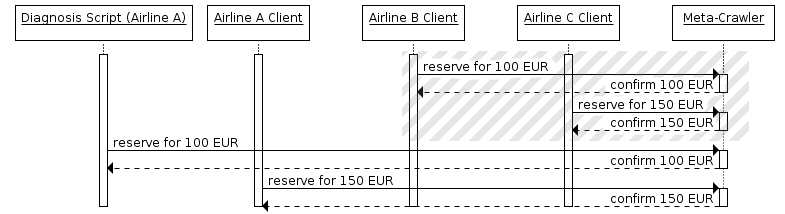
\includegraphics[width=\linewidth]{flyhehe-pass-pre-variation}
  \caption{Activity Prior To Successful Diagnosis}
  \label{fig:flyhehe-pre-booking}
\end{figure}

\subsection{Associating Variations and Assertions}
\label{sec:assoc-vari-with}

The diagnosis script is useful not only for producing similar
schedules, it also includes assertions that test the outcome of the
tested behavior. If the diagnosis reproduces a bug, those assertions
will fail.

Variances between passing and failing schedules can be used to reduce
the entry points that need to be checked for defects. If we compare
all passing schedules, we find variances that probably have no bearing
on the outcome of the test. If we compare them against the failing
schedules, and subtract the variances within the passes themselves, we
may find sequences that vary only between the passing and the failing
schedules. Those may be of particular interest to the developer,
because they are likely to be related to the failure. Such a variance
can occur in the unshaded activity in
\autoref{fig:flyhehe-pre-booking}. If the second reservation for
Airline A were sent prior to the receipt of the confirmation in the
diagnosis script, a critical race may ensue that causes the diagnosis
to fail.

Failing schedules have variances within themselves. We use this to
heuristically mark these variances as less likely causes than others,
as these variances then seem to have no impact on the outcome, since
they all produce the failure. Variances within the failure schedules
that also vary against all of the passing schedules are more likely to
be only on the path of the infected state of the program, not the
cause of the defect itself.

Consider \autoref{fig:flyhehe-failing-variation}, as an example for
variances in failing schedules. The failures, as the passes, may vary
in the order of reservations prior to the actual diagnosed
reservation---the shaded area near the top. However, the failures may
vary also in the order of the requests and confirmations for
reservations made by the diagnosis and the Airline A client---the
crossed area below. The only passing schedule for that part of the
communication is the one we see in
\autoref{fig:flyhehe-pre-booking}. Thus, the initial variances within
the failing schedule that also occur in the passes are of little
interest to the developer and need not be considered. The variances
near the end of the schedule, however, that are only between failing
schedules and do not vary within the passes can be considered likely
causes for the failure. We need to guide developers towards that part
of the communication for further debugging.

\begin{figure}
  \centering
  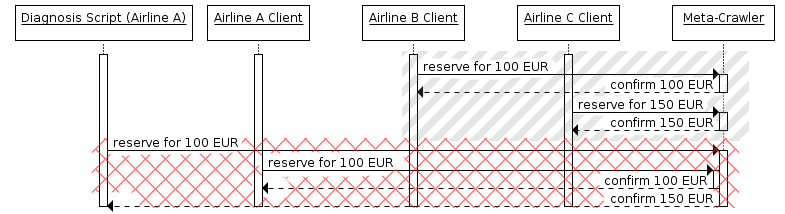
\includegraphics[width=\linewidth]{flyhehe-pass-failing-variation}
  \caption{Variations Failing Diagnosis Runs}
  \label{fig:flyhehe-failing-variation}
\end{figure}

% We could consider the interesting regions to be critical regions in
% the communication schedule, where even slight variations may cause a
% failure, and the variations that occur within passes as well can be
% considered forgiving regions of communication, where variance has
% little or no impact on the successful execution.

Finally events that occur late in the schedule are less likely to be
the original cause of a failure. To express this in our heuristic, we
adjust the probabilities linearly with respect to the sequence number
of the event within the schedule.

\section{Replay and Reordering}
\label{sec:comm-repl-reord}

Up to this point we have been inspecting the system without knowing
whether varying communication schedules are the cause for a
non-deterministic failure. We can now reinforce this assumption by
running failing schedules multiple times through what we call our
\emph{re-ordering replay scheduler}. The scheduler enforces a
particular order in network communication traces, which means we can
replay a failing trace multiple times with exactly the same order of
network events. If the result is consistently the same, even if the
failure occurred only sporadically before, we have a strong case to
believe that it was caused by this particular schedule, and further
inquiry with our method is warranted.

In some cases the outcome may vary even if our scheduler enforces a
failure schedule. An example is an improper implementation of
timestamp parsing on one machine, that causes the bug whenever the
timestamp has one of a few particular value. Such a bug will occur
regardless of the network schedule, and our approach is not suitable
to debug these kinds of failures. However, even in that case the
developer will have learned that non-determinism in the network
schedules is not responsible for the failure, and can focus his
debugging efforts on each server in turn, using traditional debugging
approaches.

\subsection{Re-ordering Scheduler}
\label{sec:re-order-sched}

The scheduler itself works as an intermediate layer between the
application code and the network, and effectively acts as a traffic
shaper\footnote{Internet standard definition of ``Shaper'' in RFC
  2475\\
  \url{http://tools.ietf.org/html/rfc2475\#section-2.3.3.3}\\
  accessed July 25, 2012}. It tries to re-order access to the shared
resource---the network---to enforce a particular, prerecorded
schedule. This is done by holding and releasing incoming and outgoing
communication according to the schedule, rather than the order in
which they arrive.

Since we want to record application layer events, it is most natural
to insert the scheduler between the application framework code
responsible for sending and receiving, and the underlying language or
operating system primitives. This has the additional advantage that
the scheduler can be programmed with some knowledge about the
framework, and thus the ability to communicate its actions to the
developer on the level of abstraction of the framework. This not only
keeps the developer in control of the debugging process, it also
allows meaningful configuration of the scheduler heuristics. Because
we record only the partial order and identifiers for communication
partners for events, the scheduler can only replay scheduled events
that occur in the system at the time of re-scheduling. That means that
\emph{all} servers that were active during record must be active
during replay as well. This may not always be the case, and scheduling
on the application layer allows us to communicate conditions for
holding and releasing events to the developers, so they can take
appropriate action, such as choosing another schedule or ensuring the
required servers are indeed online.

As an example, the scheduler can to re-order according to a schedule
that includes communication with a backup server. This backup server
may only be active at particular times of the day, say, at
night. Developers debugging a problem during the day may cause the
scheduler to wait for a long time---up until the backup server is
active. The system will seem to hang. Being able to communicate to the
developers the reason for waiting helps them to understand the
possible cause of the failure, and either bring the backup server
online for the purposes of debugging, or choose a schedule recorded at
another time.

Generally, such a scheduler has to control all points in a given
framework where application layer requests are received and
released. A possible algorithm for such a scheduler is given in
\autoref{fig:reorder-sched}. Such a scheduler will have to distinguish
whether the framework is using multiple threads of execution or just
one.

For our assumption of determinism on each server to hold,
multi-threaded servers need to be synchronized on send and receive
events, by using some kind of synchronization mechanism such as, for
example, semaphores. When a request is received, the scheduler checks
whether all requests that are expected to arrive before this request
have been received. If they have, the requests can be released into
the framework. Otherwise, the current thread of execution has to be
suspended until all previously scheduled requests have been
received. Upon release of a request into the framework, all threads
waiting on this request can be released, too. Similarly, for sending
responses, the scheduler holds those responses until all previously
scheduled responses have been sent by the framework.

Single threaded servers as they are used, for example, for event
loops, cannot be stopped if a request arrives too early, as that would
prevent any other requests from being processed. In this case, the
scheduler will receive requests into a buffer, and keep receiving
until the currently scheduled requests arrives, which is then
returned. Once the server is ready to process the next request, it may
be released directly from the buffer, if it was previously received,
skipping the network access altogether. In single-threaded mode we can
ignore outgoing requests. Under the assumption that the server works
deterministically, it will send the responses in the correct order if
it receives all requests in the correct order.

\begin{figure}
  \centering
  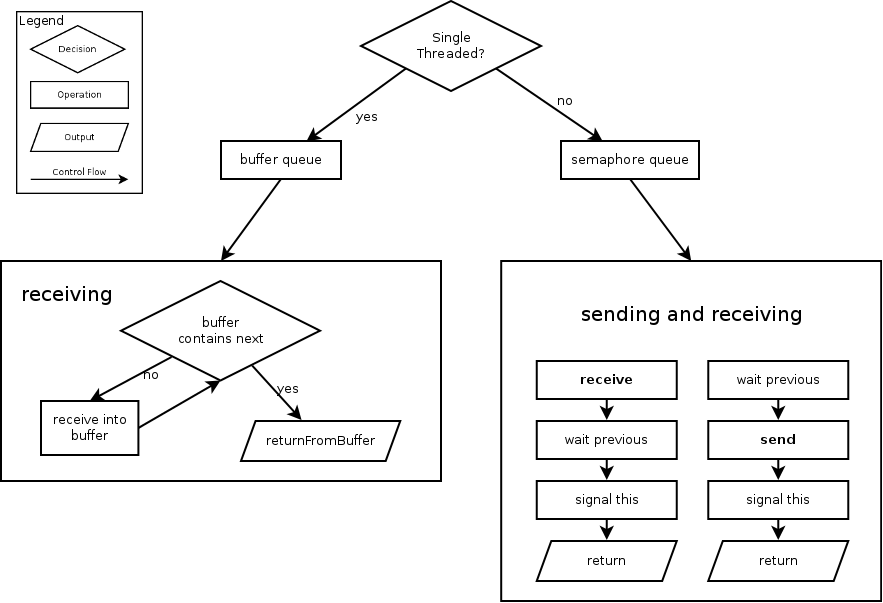
\includegraphics[width=\linewidth]{scheduler-ablaufdiagramm}
  \caption{FlowChart~\cite{Bohm1966} of Re-ordering Scheduler}
  \label{fig:reorder-sched}
\end{figure}

\subsection{Fault Navigation Over Multiple Runs}
\label{sec:replay-driven-fault}

After reproducing a failure, developers have to inspect the program
state. In \autoref{sec:lightweight-tracing} we have argued that a
lightweight logging approach is preferable for observations on the
live system, both to minimize the performance impact and the
possibility for Heisenbugs. However, this approach prohibits recording
information about the program state at this stage.

With the scheduler, however, we can enforce failure schedules as
needed for further analysis. Based on the initial communication log we
can, in a re-run, add an initial, shallow log of the called methods on
each node. This is based on the earlier work about incremental, online
analysis of runtime behavior~\cite{Perscheid2010}. Given the source
code running on the servers, this information can be connected in a
debugging tool to present a call tree to the developers.

While developers explore the call tree, it is interactively refined
on-demand. We add one-shot logging at points of interest as needed,
without disturbing the deployed system unduly. Because the the
scheduler holds on to parallel requests, the schedule will be
consistent with earlier runs and the program state will be a proper
sample.

\subsubsection{Recording the Right Data}
\label{sec:record-right-amount}

In order to assume that the observed program state for a particular
replay is a proper sample for this replay, we have to previously
record sufficient information to decide whether or not a given replay
is really equivalent to an earlier one. This means we may have to run
multiple replays for any given inquiry by the developer. Since we
record only the partial order and communication partners there is some
initial uncertainty about whether the message content is
equivalent.

Before any inquiry, we collect message samples for all communication
in a replay. This diminishes the aforementioned uncertainty, because,
on the application layer, we can treat message contents as parameters
to the remote system. This way, we can not only define a maximum
variance for messages to decide call equivalence, developers can also
review the message contents and decide, depending on the domain,
whether the schedule is correct.

\subsection{Online Replay}
\label{sec:online-replay}

In general our replay and record mechanism works for all the different
environments mentioned in \autoref{sec:observation-logging}, from
local developer setups to the deployed system. We consider the
deployed system to be the superior basis to acquire information during
replay.

A test environment already offers much better control to the
developers for debugging failures, even without the application of
Replay-driven Fault Navigation. Combined with our approach, we could
use the test environment to replace the diagnosis script with a more
"`traditional"' test, i.e a piece of executable code that resets the
test environment to a known state and then replays the recorded
live-system schedule within the test environment. Communication
partners that are part of the deployed, but not the test system have
to be mocked with prerecorded data.

The advantage of this way of using our approach is the amount of
control it offers. If the setup is sufficiently close to the deployed
system, the replay will inject the deployed system behavior into the
test environment. Multiple replays may be executed in quick
succession, as network and processing delays are small due to the
close physical proximity of servers in the test environment, and the
reduced load without live users that the system has to process, too.
Yet, those same variables may cause the test environment to produce
rare, non-deterministic failures at a different rate, or not at
all. Additionally, mocking servers that are not part of the test
environment introduces another uncertainty into the system, which
cannot be trivially proven to have no impact on the failure. Thus, we
focus on applying the replay mechanism directly to the deployed
systems.

\subsubsection{Distributed Recording}
\label{sec:distr-repl-reord}
\label{sec:distributed-scheduling}

Running debugger processes across a network and controlling them from
a developer machine introduces delays that prevent synchronous halt,
step, and resume. We circumvent these delays by using on-demand
scheduling and recording, yet, the question remains how to propagate
on-demand record in a synchronized manner in the distributed
system. We have not implemented such a mechanism, but different
designs come to mind, for the open-world case and the closed-world
case, respectively.

Our scheduler can be used to instrument some or all of the servers in
the deployed system, to replay schedules in the same environment in
which they were recorded. The advantage of this approach is the
availability of live data and more faithful reproduction of the
failure. It is non-trivial to reproduce the setup and state of a
sufficiently complex distributed system in a local test
environment. It may be easier to replay in the deployed system than to
re-create the deployment correctly enough to obtain the same execution
behavior.

In order to recover more data from the live system during replay than
we already have, the scheduler needs a mechanism specify recording
on-demand. This means that, while the developer is debugging, the
diagnosis script and scheduler replay the debugged schedule again and
again, each time recovering one more piece of information, like for
example a call stack, values of variables, and so on. Recovering only
one piece at a time means that developers have to wait until the
script has been re-executed and the information was recovered, but it
ensures minimal disruption to the service of the deployed system. This
impedes the fidelity of the approach outlined in approaches such as
the Path Tools~\cite{Perscheid2010}, which we build upon, but we show
that effective debugging is still possible with this approach
(\cf{\autoref{sec:wrapper-latency}}).

As mentioned above, our scheduler only works for well-behaved clients
in a functioning network, and in the absence of those, heuristics need
to be applied to ensure continued availability of the distributed
system overall. Since the scheduler cannot do more than wait for the
appropriate messages to appear to shape the traffic into the right
order, it depends entirely on network connectivity and deterministic
clients to reproduce a schedule. These constraints are not always met,
as network and server outages may make crucial parts of the schedule
temporarily unavailable. In this case, the scheduler will begin to
hold requests and responses on all nodes until temporary outage is
over. This is not desirable, as it effectively shuts the distributed
system down. We think that configurable heuristics for timeouts,
dropping requests or patterns for requests that should never be
rescheduled can circumvent this problem.

\paragraph{Closed-World Case}
\label{sec:clos-world-case}

In the closed-world case, all the servers in our distributed system
use our scheduler, and we have full control over the in- and output of
the system, both during record and replay. Also, no servers are added
or removed between record and replay.

During recording, each server generates a \ac{uuid} for itself, from
any suitable source such as the \textsc{mac} address of the network
card or the \ac{uuid} of other hardware components such as hard
disks. After the first execution, the log files from different servers
are aggregated into one and their \acp{uuid} are mapped to their
recorded \textsc{IP} addresses. Thus, the server \ac{uuid} allows us
to associate a server uniquely with events in the schedule.

During replay, the desired schedule is chosen at the developer
machine. The additionally desired information is added in form of
queries to the appropriate schedule event. For example, at the
beginning of a debugging session with a particular schedule, we
re-execute the schedule and for each event record the first few
hundred bytes of data sent or received. The schedule is split into
parts for each server that contributed to the original schedule and
sent out to those servers, via the same mechanism used to aggregate
the logs (\cf{\autoref{sec:mixed-environments}}). On each server the
scheduler will then read the log and re-order network access to suit
its partial schedule. Whenever an event with an additional query is
encountered, the scheduler will execute the query and log the result
before continuing its operations. At the end of each re-execution logs
are again aggregated from all participating servers and presented in
the debugger.

\paragraph{Open-World Case}
\label{sec:open-world-case}

In the open-world or mixed-world case, not all participating servers
include our scheduler or allow us to record at will---it may be
desirable, for example for Web services, to offer only replay data,
but not source code, to their developers. In the open-world case we
can also allow the number servers to change between record and replay.

In this case we record all message contents between scheduled and
non-scheduled servers. During the replay phase, any network event from
a non-scheduled to a scheduled server is performed with the recorded
data, not with the real network. The wrapped framework call for
network access is not executed. Likewise, any message sent to a
non-scheduled server during the record phase need not be sent again
during replay.

\subsubsection{Configuration Options}
\label{sec:required-heuristics}

For well-behaved clients in a closed-world setup the scheduler will be
able to perform its operation without problems, because given we start
with the right network event, all required events will eventually be
generated and the scheduler on each server can re-order events as
necessary. However, in the mixed-world case, with non-scheduled
servers, or in the face of unreliable network, with servers that
appear or disappear between record and replay---think of Web page
clients that use the deployed system while record and replay are in
progress---developers have to configure the scheduler to work under
these circumstances.

A scheduled server may receive events from servers that are not part
of the schedule, or wait to receive events from servers that were
available during record, but are not anymore during replay. We believe
this problem cannot be solved in a general way, and for these cases we
offer several settings with which developers can configure behavior
for these cases on each server.

\begin{description}
\item[Timeouts] Waiting for events may hold requests and responses
  unduly. A server that keeps no state between requests does not need
  to follow a schedule precisely for the re-execution to be
  useful. For example, in our flight reservation service, the Web page
  server has no state, as all the state is in the cache and airline
  databases. It may be useful to release network events after a
  configurable amount of time, regardless of their place in the
  schedule.
\item[Unscheduled Events] Non-scheduled servers may send events during
  replay that did not occur during record. If dropping these events is
  an option, it may be desirable to do so in order to keep the
  schedule. Otherwise, bypassing the schedule for these events may
  also work, depending on the setup---in our example clients that
  access the flight search during replay can bypass the schedule, as
  the search has no bearing on the reservation bug.
\item[Disruptions] It may be desirable to specify a separate timeout
  to wait for scheduled events. In our example the cache, which is
  queried for searches as well as rates and reservations, should not
  wait too long for an event. If a scheduled event is not generated in
  the network in time, the schedule should be marked as disrupted,
  re-scheduling is aborted, and all pending events are released. In
  this case the re-execution fails and has to be restarted.
\item[Message Level] Developers know their deployment setup best. If
  the re-execution is delayed, because the scheduler is waiting for a
  specific event to be generated from a specific server, this
  information may in itself be useful to the developers, even if the
  event never is generated. For example, if a backup is sent to
  another server from our flight cache every day at noon, and this
  caused a failure, replaying the schedule that includes the backup
  upload event can only work around noon, because otherwise the event
  is not generated. Informing the developer about this can be enough
  to provide a clue about the failure, and is preferable to stopping
  all network communication until the next backup network event is
  generated.
\end{description}

\section{Debugging at Different Levels of Granularity}
\label{sec:debugg-at-diff}

We can record and replay network schedules in the deployed system. We
use this mechanism to refining our recorded data during each
replay. The kind of additionally recorded data includes network event
contents, call stacks, method arguments, and return values. Developers
can use this information to associate events at the network
communication level to method activations at code level.

\subsection{Connecting Network Events to Code}
\label{sec:moving-from-network}

To debug asynchronously communicating applications developers need to
move between the different levels of abstraction, from communicating
servers to message sends between objects. They have to map the
observed network behavior to the original intentions expressed in the
code. In our approach we support this mapping with a tool that
integrates a network events with call trees.

One conventional approach to debugging distributed, communicating
applications is to try and determine likely locations of defects in
the code from the communication log, and the use a sequential debugger
to debug each server process independently to figure out which code
segment is responsible for a given unanticipated or erroneous network
event. However, with Web and other applications increasingly utilizing
asynchronous communication and event loops, mapping from code
locations to network events and back is becoming harder. While
outgoing requests can still be identified because they use only a
small number of framework calls for network communication, incoming
communication is increasingly handled by event callbacks. For this
style of communication, a debuggers' stack view will only reach back
as far as the last receive, with no possibility to look back further
to inspect previous communication events.

We propose tool support to provide an integrated view of both network
communication and call tree, synchronized to move freely from code to
network events and back. We argued that debugging across a network of
servers is similar to debugging across threads or communicating
objects. It appears natural to merge the communication trees and view
network communication as nested calls that originate from and return
to code. A debugging tool for distributed debugging may generally
support multiple, synchronized call trees, each call tree may show
network events or communicating objects.

Using our approach, developers are free to move through the recorded
execution both on the network level or on the code level. The
distributed debugger provides two synchronized views, one for the
global view on the network event log, and the other for a call tree
specific to the currently debugged server. Developers may interact
with the network view and, for example through clicking on an event, a
re-execution is triggered. This re-execution adds a query to the
schedule that logs all method activations on the server receiving the
event, in case of a request, or sending the event, in case of a
response. With that information, we can build an execution-specific
call tree for this server, and highlight the method activation that
was responsible for generating or receiving the network event. Since
we have recorded the full call tree, the developer is now free to move
up and down the call tree to orient himself in the code.

The debugging tool can use the information about sender and receiver
for each event to show the code that corresponds to the event. That
means showing the sender code for outgoing events and the receiver
code for incoming events. If the source code for a particular server
is available, the tool can automatically show the method responsible
for each communication event in the call tree. This provides
additional insight to the developers. They can then inspect method
arguments or local values, which will trigger additional re-executions
and recordings as needed, to find out more about how the event data is
generated or processed.

We have decided against adding support to show call trees from
multiple servers side by side, because we think the network event view
is more suitable to navigate from one server's call tree to
another. The interfaces between the different servers are encoded in
the communication data, rather than the arguments or local variables
in the servers' methods, so we think that presenting multiple call
trees side by side has no additional value.

\paragraph{Inferring Interfaces Across Languages}
\label{sec:inferr-interf-across}

A consequence of using our approach is the direct connection our
debugger can draw between code in different languages running on
different servers. Through the network events, we can infer interfaces
between those different languages. Those interfaces are implicitly
defined, in most \ac{rest} applications, or have more explicit
definitions only in another language, for example in \textsc{corba},
\textsc{soap}, or other kinds of middleware.

Without such explicit definitions so-called \ac{rest} interfaces
rarely follow a specific pattern for their communication. Oftentimes,
the wire encoding of choice is \ac{json}, because it is easy to use in
the browser and parser implementations exist for most
languages. However, \ac{json} as a simple key-value format for data
transfer offers no default interface definition language, and various
services\footnote{\xspace\hairspace
  Github API v3: \url{http://developer.github.com/v3/}\\
  Twitter REST API: \url{https://dev.twitter.com/docs/api}\\
  accessed July 25, 2012} offer no more than textual descriptions and
examples for their \ac{rest} \acp{api}. Such descriptions are hard to
verify against an implementation.

The more immediate issue with informal descriptions of \acp{api} is,
however, that outdated information is difficult to update, as this
requires checking the source code and update the documentation with
the informal \ac{api} description. With our approach, the interface
can be determined without access to the source code, by reviewing
recorded message contents for valid communication. If there is a
communication error somewhere in the log, and it is suspected to be
due to improper usage of the \ac{api}, the event's message contents
need only be compared against a log of a working communication, to
test this hypothesis.

Once such an error is discovered, our approach offers the direct
connection from the problematic events to the source code where the
events are generated and received. Thus, developers can test their
hypothesis and move to the appropriate piece of code to fix a
potential problem.

%%% Local Variables: 
%%% mode: latex
%%% TeX-master: "thesis"
%%% End: 

\chapter{Implementation}
\label{cha:implementation}

\begin{figure}
  \centering
  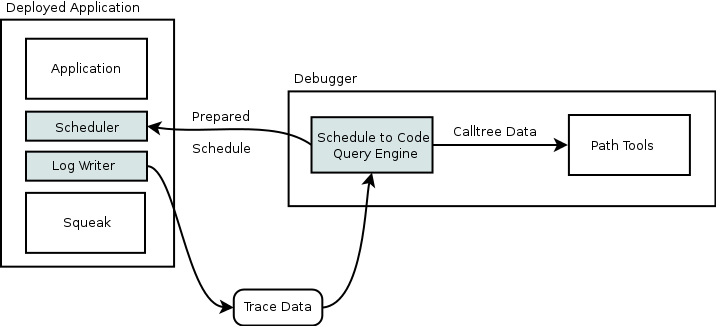
\includegraphics[width=0.9\linewidth]{structure}
  \caption{Interactions in the Prototype}
  \label{fig:structure}
\end{figure}

We evaluated our approach in a prototype for distributed applications
using \ac{http} to communicate, implemented in
Squeak/Smalltalk~\cite{Ingalls1997}. In this chapter, we explain how
we hooked into the entry and exit points for network communication,
for which we used \emph{ContextS}~\cite{Hirschfeld2008}, an
implementation of \ac{cop} for Squeak/Smalltalk. We already mentioned
that we built on earlier work about online analysis of runtime
behavior, implemented in the \emph{Path Tools} suite, and we have
based our debugging tool and visualization on the Path Tools
suite. \autoref{fig:structure} shows how our protoypes' components
interact. Applications are instrumented with ContextS to include a
logging and a scheduler layer. The logging creates trace data that is
used by our query engine to display the network communication patterns
with the Path Tools and provide any recorded call tree data. When the
developer chooses a schedule for re-execution, queries are attached to
the schedule events, the prepared schedule is sent to the scheduler,
and the application is re-executed. The scheduler shapes the
communication during re-execution to match the schedule and records
any additional information using the same mechanism as the log
writer. The resulting trace data is again sent to the query engine,
which passes the newly recorded information to the Path Tools for the
developer to inspect.

\section{Tracing Communication Patterns}
\label{sec:trac-comm-patt}

One way to implement the logging of logical communication schedules is
tracing the appropriate code executions in the system. For our
application, we identified the methods in a Squeak image where
\ac{http} requests are received and responses are generated. Our
example application used, besides the standard library \ac{http}
communication, the \emph{KomHttpServer} for receiving requests.

Tracing communication at different levels of granularity was vital to
verify our approach in a prototype. We chose ContextS so we could
easily add various layers with different logging mechanics for
experimentation. Additionally, ContextS layers are easy to manage in
Monticello, the \ac{vcs} of Squeak. This allowed us to keep the
tracing implementation as a separate project an thus fairly
independent of the traced system.

The combined log includes all events that were recorded between two
particular points in time. These points in time are given by the start
and finish of our diagnosis to reproduce a failure. Re-executing such
a diagnosis a number of times yields different time slices of
communication. We present these logs in a diagram with events as data
points and logical time on the x-axis. Because events are data points,
and there may be many events in one schedule, our visualization scales
all events to fit into one window. For many events, this allows
developers to get a high-level overview of the activity throughout the
system without swamping with detail. In \autoref{fig:comm-overview} we
see such an overview. While we cannot make out details, we can see
that the service running on \emph{localhost} port 5001 is active more
consistently than the one below it, running on port 5002. This
high-level pattern communication pattern may already provide some
insight as to how the system works.

\begin{figure}
  \centering
  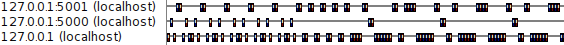
\includegraphics[width=0.95\linewidth]{comm-overview}
  \caption{Communication Schedule Overview}
  \label{fig:comm-overview}
\end{figure}

\autoref{fig:comm-logs} shows an example of a very small communication
schedule. We show the number of diagnosis runs that yielded this
particular schedule (\textcircled{1}), and how many events there are
in this schedule. The color of the box shows whether there were any
errors, such as failed assertions, during the diagnosis' execution by
turning from green to yellow. The recorded communicating servers
(\textcircled{2}) are presented as \textsc{IP} address labels on the
y-axis, with the associated port (if any). If that address resolves to
a host name, it is added in brackets. \emph{Lifelines} extend from the
endpoints, so events on the right-hand side can be easily associated
to a particular server. Each box represents an event with outgoing
events (\textcircled{3}) in red and incoming events (\textcircled{4})
in blue. The boxes in this visualization represent a point in time
rather than a time span, and their width is simply as wide as possible
to still show all events within the graph. Because each box shows the
first few bytes of captured message data if such has been captured, it
is useful to have boxes as wide as possible.

\begin{figure}
  \centering
  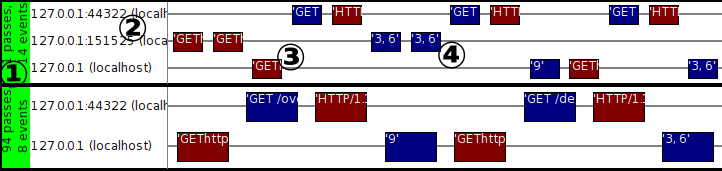
\includegraphics[width=\linewidth]{comm-log}
  \caption{Captured Communication Logs}
  \label{fig:comm-logs}
\end{figure}

\subsection{Distributed Context-oriented Computing}
\label{sec:distr-cont-orient}

ContextS layers can be dynamically enabled and disabled to extend
methods at runtime. For a distributed system, these layer activations
have to be distributed across the network, so enabling a particular
tracing mechanism on one system carries over to another. This can be
achieved in various ways. Because our layers are implemented for
\ac{http} requests only, we decided to propagate layers in a custom
\ac{http} header, \texttt{X-DCOPActiveLayers}, an application specific
header in accordance with RFC 2047. This header contains not the names
of the currently active layers, but, as suggested in~\cite{Rho2011},
an ontology describing those layers. This decouples the layer names on
our particular implementation from possible other implementations and
their layer names, by describing what layers do instead. Those headers
will be ignored by conforming implementations that do not use our
tracing package. On systems that do use our tracing, we read the list
and activate the layers globally as required.

Most Web application frameworks employ the \emph{inversion-of-control
  principle}, which does not work well for ContextS. In ContextS,
layer activations are valid for the dynamic scope of the execution,
and do not propagate upwards the stack from the point of
activation. This problem with \ac{cop} in the context of
inversion-of-control frameworks is known and has been treated in
recent work~\cite{Appeltauer2012,Appeltauer2012Phd}. We have not
implemented the mechanism to deal with this problem, so our prototype
is not able to activate layers across the network. Rather, the
required layers are simply active all of the time.

In related work, DejaVu uses a similar mechanism on the transport
layer that involves embedding and, on the remote end, stripping magic
bytes in \ac{tcp} packages~\cite{Konuru2000} to propagate
meta-information for tracing.

\subsection{Tracer Entry Points}
\label{sec:tracer-entry-points}

Tracing \ac{http} requests with ContextS entails finding and layering
methods in frameworks and standard library that create and receive
\ac{http} requests. In our example, using the Squeak standard library
and the KomHttpServer framework, this included layering only 3
methods.

Extending the implementation to work for other Squeak Web servers or
other application layer frameworks such as relational database
adapters is trivially possible. The actually captured data only
includes the local logical timestamp, as well as the sender and
receiver of the message.

\subsection{Trace Format}
\label{sec:trace-format}

To actually implement our approach for different runtimes and debug
across languages, an interchangeable trace format is necessary. We
have not implemented such a format. Our prototype is Squeak-based, so
the interchange format consists of a Squeak store string, which can be
recompiled into a collection of trace events. Each trace event, here,
is an object with a logical timestamp, receiver and sender \textsc{IP}
and port.

An interchangeable trace format is trivial to implement, however. To
exchange logs, we only need a way to transfer collections of event
3-tuples that include strings and integers which almost any
data-interchange format should be able to. \ac{json} seems to be a
natural choice, both because it is widely used and parsers are readily
available for a variety of languages, and because it is the most
common format in Web development.

\section{Communication Diffing}
\label{sec:diff-comm}

As per our design (\cf{\autoref{sec:comm-constr-analys}}), we regard
each communication schedule as a sequence diagram with only
asynchronous message sends. To help developers find differences in the
schedule, we want to automatically differentiate traces to show areas
of high and low variance in the schedule. For $N$ servers, at any one
logical time, there are at most $N$ network events. Comparing
different communication schedules can thus be done by comparing each
logical time in order, similar to how a patch algorithm compares files
at different versions.

\subsection{Difference Format and Visualization}
\label{sec:diff-form-visu}

The choice of algorithm for automatic differentiation can have a huge
impact on the usefulness of the result. There are various algorithms
to differentiate tree structures~\cite{Bischof2008AiA}. We treat our
communication schedules as call trees with only asynchronous
communication. That means they can be transformed into a linear form,
which makes them suited for the linear differential algorithms used
for file comparison. Of those, we chose the \ac{lcs} algorithm to
create differential schedules.

We can assume that schedules will vary in some events or
event-sequences, but will be equivalent for some length around those
variances. \ac{lcs} dynamically finds the longest matching
sub-sequence between two pieces of data. For comparing two schedules,
we choose one as the \emph{base} and the other as the change. In
\autoref{fig:comm-diff} we show such a differential schedule between
the base at the top and the comparison schedule at the bottom.

The differences between the schedules are marked in red. If we compare
the overall number of events, we can see that both the base schedule
at the stop and the comparison schedule at the bottom have the same
number of events. They are equivalent up to the first red marker,
where the comparison schedule sends out a \texttt{GET} request that
does not occur in the base schedule. If we follow the differential,
however, we can see that the schedules are equivalent again for four
more events until the second red marker. At that point, a \texttt{GET}
request sent in the base schedule does not occur in the comparison
schedule. Afterward, both are equivalent up to the end.

\begin{figure}
  \centering
  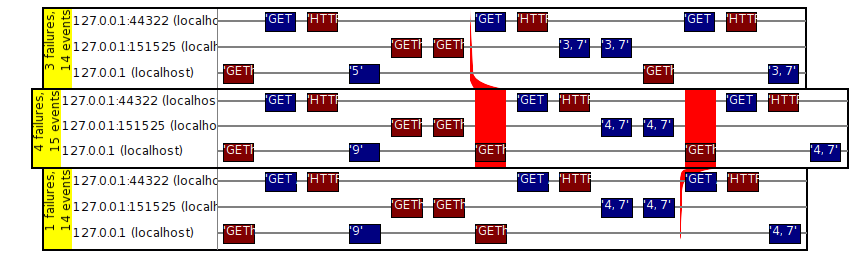
\includegraphics[width=\linewidth]{comm-diff}
  \caption{A Simple Differential Between 2 Schedules}
  \label{fig:comm-diff}
\end{figure}

\subsection{Correlating Variances and Failures}
\label{sec:corr-vari-fail}

Not all variances will usually contribute to the failure, yet, for
large numbers of runs we may have more variances than common
sub-sequences. Simple red/white differentials are not very helpful in
this case, as they do not significantly reduce the search space to aid
developers in their search for the problem. Due to this, we weigh
variances according to a number of rules, which have been in described
in \autoref{sec:assoc-vari-with}.

The heuristic probability distribution is mapped onto hue values from
zero to sixty degrees, which corresponds to full red and full yellow,
respectively. For variances that the heuristic recognizes to have no
impact on the failure, we assign the color gray.

To review variances between passing runs, we assign hue values
depending on the amount of variance on each particular network
event. The function \emph{hue}, below, shows how we map the each event
onto a range from 0 to 1. We then map this range onto a range from 0
to 60, corresponding to the colors from red to yellow in the
\textsc{hsl} color space. We assign alpha values from 0 to 1
accordingly, which means that events with a hue closer to 60 are
hardly visible.

\begin{align*}
  \label{eq:1}
  T & = \text{set of trace event sets} \\
  N(event) & = \{ T_{i} \in T | event \in T_{i} \} \\
  P(event) & = \{ T_{i} \in N(event) | T_{i} \text{ is pass} \} \\
  hue(event) & = \left\{
    \begin{array}{l l}
      \left(1 - \frac{|N(event)|}{|T|}\right)^2 & \qquad \text{if } N(event) = P(event) \\
      \sqrt[12]{\left|0.5 - \frac{|P(event)|}{|N(event)|}\right|} & \qquad \text{else}
    \end{array}
  \right.
\end{align*}

The result of this mapping, shown in \autoref{fig:hue-mapping}, is
that high-variance events from traces that are all passes or all
failures show more red, which in return means that low-variance events
have almost no highlighting. In sets of traces that include both
passes and failures, the second branch of the \emph{hue} function is
used to determine a value that highlights events that occur not in all
passes---thus are not likely to be the cause for passing---but also
not only in failures.

\begin{figure}
  \centering
  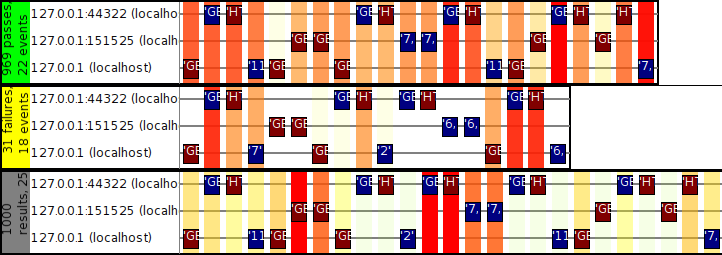
\includegraphics[width=\linewidth]{hue-mapping}
  \caption{Hue Mapping For Events}
  \label{fig:hue-mapping}
\end{figure}

\section{Reordering Access to Network Resources}
\label{sec:reord-access-shar}

In our prototype we support re-scheduling network access in the live
system. Parallel network events inherently cause races, the network
transport may transmit messages at different speeds and the operating
system may forward messages to user space applications as it sees
fit. To reorder access to network resources, the network events have
to arrive at the application in order, so network events have to be
re-ordered in a layer between the application and the hardware.

We decided to re-order events in the language, using the same
mechanism as for tracing. We use ContextS to define a scheduler layer
between applications and the KomHttpServer framework and the Squeak
standard library (\cf{\autoref{fig:structure}}). This scheduler layer
is only active if a schedule was requested.

\subsection{Constraints on the Networked Systems}
\label{sec:constr-netw-syst}

Our design is supposed to work for local systems on the developer
machine, in test environments and the live system. However, because we
only record communication partners and the partial ordering of events,
in practice, there are various constraints on those systems. First,
hey have to be deterministic in their communication, which means if we
send them messages in the right order, they return valid responses in
right order. This means have to be able to control the order in which
messages are received. However, with systems that employ load
balancing, multi-threading and event loops which are designed to
handle multiple requests in parallel we cannot be sure that for
multiple requests the responses are generated in order. This means we
have to control the send order, too.

\subsection{Entry Points}
\label{sec:entry-points}

According to the design, there are two types of entry points which we
need to control to enable re-scheduling, both for sending and
receiving. We only deal with \ac{http} requests and, because we use
the same context-oriented mechanism as for the tracer, we only had to
create a layer to wrap the same three methods as for the tracer. Our
scheduler layer is always active and the wrapper methods check whether
a schedule was requested. This check simply uses a globally available
singleton object and checks whether it contains a valid schedule. If
not, the scheduler methods do nothing and simply proceed.

\subsection{Scheduling Execution}
\label{sec:scheduling-execution}

Our implementation follows the design shown in
\autoref{fig:reorder-sched}. The framework we used to implement our
example application uses threads to handle multiple connections, so
for simplicity, we have only implemented the threading scheduler using
semaphore queues.

To schedule an execution, the trace that is used as basis for the
execution is copied and transformed into a list of schedulable
events. All of these events contain the identifiers for the original
communication partners, the id of the event and a semaphore in the
\emph{waiting} state. This list is then attached to the globally
accessible singleton object and the first semaphore is
signaled. Finally, the diagnosis script is started to provide the
required events.

\paragraph{Receive}
\label{sec:receive}

The KomHttpServer uses a blocking \emph{accept} call on a socket
object to wait for incoming requests, which the \ac{vm} translates
into the \emph{accept} system call. When that call returns, the
operating system socket has data available. The KomHttpServer
framework then spawns a new thread that creates an
\emph{HttpRequest} object from the received data and passes this
into the application.

Before it passes from framework to application code it has to go
through our scheduler. The scheduler uses an atomic operation to find
the appropriate event in the schedule for this request, attach the
request object onto it, and return the event object from the
schedule. It then calls \emph{wait} on the event object's
semaphore. If the semaphore was already signaled this call returns
directly, otherwise this thread blocks until the semaphore is
signaled.

When the \emph{wait} call to the semaphore eventually returns, the
semaphore for the following event is signaled and the request object
is passed back into the framework, from which it passes on into
application level code.

\paragraph{Send}
\label{sec:send}

Sending of data works similarly. The application manufactures an
\emph{HttpResponse} object and returns it to the framework. The
framework the calls the \emph{writeOn:} method with the socket object
to serialize the response onto the socket stream. We wrap this method
and use the atomic find, set, and return operation on the schedule to
find the scheduled event corresponding to this response, and then wait
on the semaphore. When semaphore is signaled, we proceed to the base
method which writes the response to the network.

The fact that we have only implemented the semaphore list for our
scheduler means that means it is currently limited by the maximum
amount of threads available to the framework for handling multiple
connections. Because each thread blocks if the event cannot be
released directly there may be situations in which so many threads are
blocked that the framework cannot create any more threads for incoming
requests, at which point the server will deadlock. We circumvent this
problem in our implementation by having the semaphore wait time out
after a configurable amount of time, after which point the
re-scheduling deviates from the desired schedule.

\subsection{Probable Replay}
\label{sec:probable-replay}

A goal for a scheduler following our design is to enable consistent
replay. Our design only works for well-behaved clients and stable
networks, constraints that cannot always be guaranteed in a real
environment. However, these constraints may often be met, even if not
all the time. A practical re-scheduler may not always work, but it
raises the probability that a specific schedule will be reproduced,
and it will reproduce the schedule if the circumstances permit. If the
network is sufficiently disturbed, either because of misbehaving
clients or connection problems, the scheduler deals with it by
deviating from the desired schedule.

As mentioned above, our implementation uses timeouts to make sure that
the distributed system does not lock up, but timeouts include the
potential for releasing events too early and thus deviate from the
desired schedule, causing a re-execution inconsistent with the
original trace. Our implementation also continually checks for
disturbances defined in
\autoref{sec:required-heuristics}---unscheduled events, schedule
disruptions by misbehaving clients---and we have implemented
configuration settings that determine how we deal with them. These
settings currently allow developers to choose to drop unscheduled
events, or pass them through without waiting for a semaphore. Our
implementation additionally uses simple printf logging to communicate
to the developers how it is reshaping the network schedule, i.e. which
events have been encountered, which are being waited for, and which
disturbances were encountered and how were they dealt with.

\section{Connecting Network and Object Communication}
\label{sec:conn-netw-object}

Adequate tools are essential for efficient debugging. Previous
approaches at efficient replay for the most part focus on recording
and replaying correctly and efficiently, but use existing debuggers
like \emph{GDB} for interactions with the program state, and separate
tools to review the captured network data. Other approaches, like
\emph{Causeway}, focus on the tools.

We think that the debugging tool should be integrated, allowing the
user to inspect both object and network communication in one view, as
they are in Causeway. However, efficient replay is required for those
tools to be practical, so a recording and replay mechanism like our
scheduler has to be integrated into the tool.

Our prototype extends the call tree view, called \emph{Path Finder},
which is part of the Path Tools suite. Our tool, inspired by Causeway,
shows network communication and the call tree for one server in a
single window. These views should be synchronized, so if a user opens
a method, the closest network event should highlighted. Inversely,
clicking on a network event should open the call tree on the method
that is closest to the network event. If the network event was sent or
received on the server to which the call tree belongs, it should show
the method responsible for the event.

For this prototype, we have only implemented moving from the network
to the code view, not vice-versa. If a user clicks on a network event,
the scheduler is instructed to record the stack at the time of the
network event and the test case is re-executed. We then search for a
method on the stack that is part of our call tree, and open that
method for inspection. In \autoref{fig:pathfinder} we show the result
of clicking on the third network event~\textcircled{1}. In the lower
part of the window, the call tree is expanded to the method which sent
the event.

\begin{figure}
  \centering
  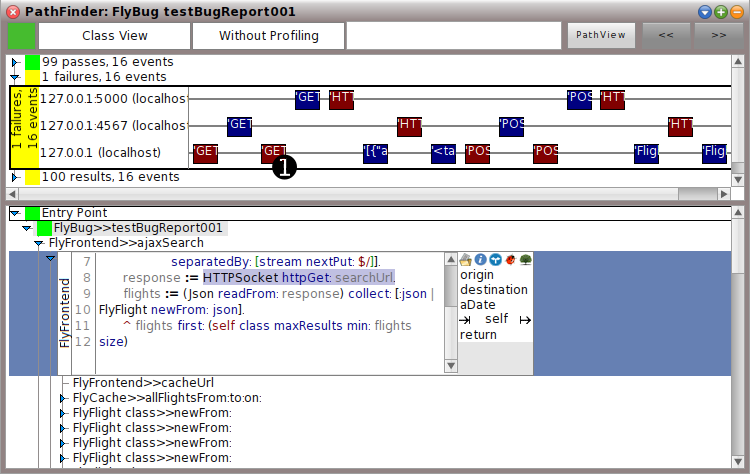
\includegraphics[width=0.9\linewidth]{pathfinder}
  \caption{The Path Finder Network Extension}
  \label{fig:pathfinder}
\end{figure}

A full implementation should support full synchronization between the
two views. We have also not implemented additional queries of the
program state. A fully implemented tool should support queries of
single variable values, method arguments and other program state in
the scheduler, to allow further inspection of the program state.

%%% Local Variables: 
%%% mode: latex
%%% TeX-master: "thesis"
%%% End: 

\section{Evaluation}
\label{sec:evaluation}

\todolist{tim}{
\item show Sudoku constraints 
\item explain constraints
\item add multiplayer events with constraints (to demonstrate how a
  new codepath does not break the system and ``just works''}
  
  
This section evaluates how well constraint applications with Babelsberg/S facilitate reactive systems.

We argued that logic puzzles, like Sudoku puzzles, are good examples for interactive constraint applications. Therefore, the evaluation uses Sudoku as example application. In \autoref{lst:sudoku-constraints}, you will find all necessary constraints to solve a Sudoku puzzle.

\begin{lstlisting}[caption=All Constraints of a Sudoku Puzzle, label=lst:sudoku-constraints]
sudoku addConstraintsForAllGivenNumbers.

[sudoku allSatisfy: [:cell | cell between: 1 and: 9]] 
		alwaysSolveWith: solver.
		
(1 to: sudoku rowCount) do: [:index |
		[(sudoku atRow: index) allDifferent &
		(sudoku atColumn: index) allDifferent &
		(sudoku atBox: index) allDifferent] 
				alwaysSolveWith: solver].
\end{lstlisting}

The second one, line 3 and 4, was already explained in \autoref{sec:ocp_squeak}. The first line adds equality constraints for all given numbers, so that the constraint solver cannot change them. In general, they are called stay constraints, which are currently not supported in Z3, but will be in future versions. The last constraint, line 6 to 10, describes that all numbers in each row, column and box, are different. The keyword for that is \texttt{allDifferent}, which is a new collection method in Babelsberg/S. Together, the second and third constraint say that each row, column and box contains all numbers from 1 to 9.
\chapter{Related Work}
\label{cha:related-work}

Because our approach combines work in various areas of distributed
systems debugging, from continuous record and replay, over
replay-driven fault navigation, debugging at different levels of
abstraction and full-on distributed debugging, we have sub-divided our
treaty of related work in this chapter into sections for each of those
domains.

\section{Record and Replay}
\label{sec:record-replay}

The need for consistent record and replay to debug certain kinds of
distributed applications is widely accepted. Approaches vary mainly in
how much they record, and subsequently how much of the system they can
simulate to eliminate behavioral disturbance.

\paragraph{Replay with Mocks}
\label{sec:replay-with-mocks}

Mocks are program entities designed to simulate the behavior of a real
entity. In system replay, mocks may be used to stand in for network
nodes. If enough information about the data sent by a particular node
has been recorded, there is no need to re-execute that node during
replay. Assuming the node works deterministically, a mock can return
the appropriate responses.

This approach is advantageous for nodes that are not under debugger
control. On those machines, package races on the network cannot be
rescheduled upon receive and behavior may still vary during
replay. Mocks avoid that problem, at the cost of greater recording
overhead at least in space, if not in time, for copying message
contents.

We have opted not to use mocks in this work, but other approaches use
mocks for some or all the nodes during a replay.

\paragraph{Deterministic Replay on the JVM with DejaVu}
\label{sec:dejavu}

\emph{DejaVu}~\cite{Konuru2000} is a record and replay framework for
distributed Java applications. It uses modified \acp{jvm} to execute
java applications and record their thread schedules as well as network
access. Thread and network schedules use implementations of Lamport
Clocks to establish event order.

The level of abstraction for network events in DejaVu is lower than in
this work, recording \ac{tcp} instead of \ac{http} events. While this
enables replay just as well, we argue that it is harder for a
programmer to review \ac{tcp} traffic and connect it to the program
domain than it is with \ac{http} events.

Contrary to this work, DejaVu supports both open and mixed world
record and replay. we note in \autoref{sec:distr-repl-reord} how the
same may be accomplished in my implementation.

\paragraph{Tracing and Simulation with iDNA}
\label{sec:idna}

\emph{iDNA}~\cite{Bhansali2006} is part of Microsoft-developed
framework for instruction-level tracing and replay of applications in
user-mode. The solution includes running instrumented programs atop a
runtime called \emph{Nirwana}, which provides hooks for iDNA to
register points of interest for tracing. The Nirwana runtime uses
dynamic binary translation to break a monitored process' instructions
into smaller instructions that are then instrumented and executed on
the host. The iDNA tracing component records traces via callbacks from
the Nirwana framework and, for replay, reads trace records and feeds
Nirwana desired instruction pointer and register values for
replay. The overhead is about one order of magnitude, which makes it
feasible to run IO-bound applications in tracing mode all the time,
which is also the scenario envisioned by the authors.

Due to its low level of recording, iDNA supports multi-threaded
applications, as well as applications that generate executable code at
runtime, such as \ac{jit}-compiled languages, but does not target networked
applications specifically. Similar to the present work, iDNA is aimed
at tracing continually on the live system, but the focus is on single
process applications rather than communicating processes or servers.

\paragraph{Reproducible Failures with ReCrash}
\label{sec:recrash}

\emph{ReCrash}~\cite{Artzi} is a framework to observe program execution in
Java and generate test-cases that reproduce observed errors. Similar
to this work, it can be applied to live systems. ReCrash does not try
to preserve enough information to replay an observed failure from the
beginning, but rather just keep enough information around to provide
an method entry point with arguments that trigger the crash.

To do this, ReCrash keeps a \emph{n}-deep \emph{shadow stack} during
execution with copies of the receivers and arguments. If a crash
occurs the stack is saved. In a second step, the shadow stack is
searched for the first call that reliably reproduces the exception.

The ability to reproduce crashes using this technique is limited by
the size of the shadow stack, as well as the copy depth of receiver
and arguments at each stage. Deeper stack and copying might be more
able to reproduce a crash, but imposes a larger overhead. The authors
offer a way out by only enabling monitoring after a crash occurred for
the first time, and only for methods on the stack at that point. Since
in this mode \emph{no} information has been saved about the execution,
the crash has to occur again, which might take a very long time for
rare exceptions.

For the class of problems that are related to causes that are not on
the same stack, like the concurrent update problem presented in this
thesis, ReCrash has only limited value.

\paragraph{Output-deterministic Replay with liblog}
\label{sec:liblog}

The \emph{liblog}~\cite{Geels2006Replay} tool for distributed C/C++
applications uses a {\tt libc} wrapper library to intercept system
calls and record events such as network communication, file access,
and \ac{ipc}.

The goal, as in this work, is to record sufficient information in the
live-system to replay execution at will for later debugging. The
authors decided against \emph{in-situ} replay, however, and use a
central console to download all logs and program checkpoints to
re-instantiate the program locally. Additionally, they record enough
information to replay each process independently of the others, which
imposes a higher tracing overhead.

Like DejaVu, and unlike this work, liblog records events at a very low
level. Most programs written for the Web, for example, do not use
socket programming directly, so the programmer will still have to
match the recorded network communication to the level of abstraction
in his code.

\section{Replay-driven Fault Navigation}
\label{sec:replay-driven-fault-1}

\paragraph{Test-driven Fault Navigation with Path Tools}
\label{sec:pathtools}

The \emph{Path Tools}~\cite{Perscheid} are a research project in
Squeak/Smalltalk and the basis for our prototype. Path Tools uses
re-executable entry points, mostly tests, to exercise code paths in a
project for analysis. These entry points need to execute
deterministically in order for the Path Tools' analysis to work
correctly.

In our work we have extended Path Tools and use it for re-execution
and analysis of distributed applications. Because Path Tools currently
need deterministic execution paths to work, this work offers an
approach to make network communication deterministic.

\section{Debugging at Different Levels of Abstraction}
\label{sec:debugg-at-diff-1}

\paragraph{Network Analysis and Debugging with Firebug}
\label{sec:firebug}

\emph{Firebug}\footnote{Mozilla Firebug:
  \url{http://getfirebug.com/}\\
  accessed June 20, 2012} is an open-source debugger and Web
application analysis tool for \emph{Firefox}\footnote{Mozilla Firefox:
  \url{http://www.mozilla.com/}\\
  accessed June 20, 2012}. It offers a JavaScript debugger with
breakpoints and a network pane to review \ac{xhr} requests made from
the JavaScript code of the web-page. Firebug includes the ability to
log network communication and set breakpoints on incoming and outgoing
connections, which enables developers to move from network to source
code, but not the other way around.

Firebug, like traditional debuggers, works synchronously on the code
and network communication of the current Web pages' JavaScript
process, and offers no integration with other services or debugger
instances. Also, while it is possible to break on network events and
move to the source code callback for a given event, there is no
further integration between the two~\cite{Barton2010}.

\paragraph{Message-oriented Debugging with Causeway}
\label{sec:causeway}

\emph{Causeway}\cite{Stanley2009} is a message-oriented debugger that
tries to unify the network request/response view with the message
send/receive view of the software. The authors' approach is to trace
program execution as well as network communication partners and
message contents, and present the captured information in a
post-mortem debugger. This debugger synchronizes the network and the
stack view so moving in one will update the other
(\cf{\autoref{fig:causeway}}), a behavior which has been the main
inspiration for how we show the two levels abstraction in our
prototype implementation.

In difference to this work, Causeway is strictly post-mortem. That
means it has to trace all required information, all the time, imposing
a very high overhead, a problem the authors mention themselves.

\begin{figure}[h]
  \centering
  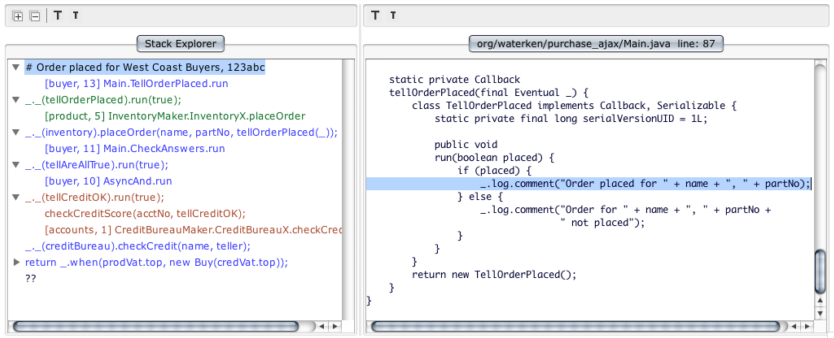
\includegraphics[width=0.7\linewidth]{causeway}
  \caption{Causeway Message Debugger}
  \label{fig:causeway}
\end{figure}

\section{Distributed Debugging}
\label{sec:distr-debugg}

Most debuggers work one thread at a time, and only for one process,
and offer the programmer a way to switch threads while debugging. Most
debuggers allow developers to stop all threads at once, however, this
disturb the execution order and lead to heisenbugs, since uniformly
starting and stopping multiple threads is not possible, even within a
single process. This equally applies to processes that are distributed
across a network. However, some runtimes, such as the \ac{jvm} or the
\ac{clr}, but also distributed systems middleware, such as
\textsc{corba}, still allow developers to stop and inspect processes
across a network.

\paragraph{Virtual Machine Interfaces on JVM and CLR}
\label{sec:java}

Both the \ac{jvm} and the \ac{clr} offer debugging facilities to
connect symbolic debuggers to remote processes. These facilities, in
case of the \ac{jvm} using a custom \ac{jvmti}\footnote{\textsc{jvm}
  Tool Interface Version 1.0\\
  \url{http://docs.oracle.com/javase/1.5.0/docs/guide/jvmti/jvmti.html}\\
  accessed July 31, 2012} and in case of the \ac{clr} built on the
\ac{com} standard~\cite{Strein2005}, abstract from the network to
offer the same debugging experience across a network as for local
processes. Debugging multiple processes from the same \ac{vm} is
possible with these approaches. Additionally, both of these \acp{vm}
are built to support different languages, so debugging across
languages is possible, too. However, we know of no debugging tool for
either \ac{vm} that supports different languages.

Compared to this work, these debugging interfaces have two
shortcomings: first, to inspect a remote process that process has to
be stopped by the debugger. It is undesirable for a deployed system to
stop providing its service because a debugger is connected to
it. Second, these debugging facilities only provide a view on the
program, and do not track network communication between processes, so
it is still difficult to get a global view of the distributed system.

\paragraph{Debugging Distributed Objects with CORBA and SOAP}
\label{sec:corba}

As a logical extension of object oriented programming into the realm
of distributed systems, middleware layers, such as
CORBA~\cite{Yang1996} and SOAP~\cite{Walsh2002}, have evolved. They
allow developers of distributed systems to specify object interfaces
for publishing and accessing distributed services in an
interchangeable format. Developers can program against these
interfaces as if the distributed system were running in a single
process, while the middleware takes care of communication. However,
much of the development time complexity hiding provided by middleware
is lost when debugging, because developers cannot step into message
sends that are converted to network communication by the
middleware. Recently, effort has been expended to enable symbolic
debuggers to overcome this restriction and step across
servers~\cite{Mega,Kaler2007} when debugging on top of such
middleware.

Such debuggers for middleware systems, like the middleware systems
themselves, try to abstract from the network. Approaches at stepping
across servers are extensions to symbolic debuggers that are meant to
allow developers to inspect objects in distributed system as if they
were locally available. In contrast to this work, these debuggers
target systems that are fully under developer control and can be
stopped at will for inspection. Like traditional symbolic debuggers,
they ignore Heisenbugs caused by the debugging process and are not
well suited to debug non-deterministic failures.

%%% Local Variables: 
%%% mode: latex
%%% TeX-master: "thesis"
%%% End: 

\section{Conclusions}
\label{sec:conclusion}

\todolist{tim}{
\item constraints are useful to write reactive systems
\item the relationships between objects are modularized
\item adding new codepaths that affect the relationships works
  automatically}
  
%% softened the conclusion a little - I don't think we have shown this
%% conclusively yet
We have argued that \ac{ocp} facilitates reactive systems, because it
modularizes the relationship between objects and decouples constraint
satisfaction from the application.  In Babelsberg, constraints can be
dynamically added and removed and maintained automatically, making
them useful for writing interactive applications.  As an example, we
implemented an interactive application for specifying and solving a
Sudoku with constraints.  With the interactive \ac{gui}, the user can
change the values of the constraint variables without breaking the
properties of the Sudoku.  The application reacts on the user input by
resolving the underlying constraints.
%%% Local Variables:
%%% mode: latex
%%% TeX-master: "paper"
%%% End:


\printbibliography
\clearpage
\appendix
% % !TEX root = Stolpe_2018_Thesis.tex
% !TEX encoding = UTF-8
%% ggf:
% \part{Appendix}
% \label{part:appendix}

\chapter{First Unimportant stuff.}
\label{cha:first-unimp-stuff}

\blindtext
%%% Local Variables:
%%% mode: latex
%%% TeX-master: "Stolpe_2018_Thesis"
%%% coding: utf-8
%%% End:

\backmatter
\markboth{}\relax
\ifthenelse{\boolean{thesis}}{
% \clearpage
% \null
\cleardoubleemptypage
\ifxetex
\begin{german}
\else
\begingroup
\selectlanguage{ngerman}
\fi
  \dateselectlanguage{german}
  \setdatebynumber{\thedatenumber}
  \chapter*{Eigenständigkeitserklärung}
Hiermit versichere ich, dass ich die vorliegende Arbeit selbständig
verfasst sowie keine anderen Quellen und Hilfsmittel als die angegebenen
benutzt habe.\\[7\baselineskip]
%
  Potsdam, den \datedate \hfill \rule{.45\textwidth}{0.4pt}\par
%
  \raggedleft \makeatletter\@author\makeatother\par
\ifxetex
\end{german}
\else
\endgroup
\fi
%%% Local Variables: 
%%% mode: latex
%%% TeX-master: "thesis"
%%% End: 


}{}
% \listoftodos
\end{document}

%%% Local Variables: 
%%% mode: latex
%%% TeX-master: t
%%% End: 
